%%%%%%%%%%%%%%%%%%%%%%%%%%% asme2ej.tex %%%%%%%%%%%%%%%%%%%%%%%%%%%%%%%
% Template for producing ASME-format journal articles using LaTeX    %
% Written by   Harry H. Cheng, Professor and Director                %
%              Integration Engineering Laboratory                    %
%              Department of Mechanical and Aeronautical Engineering %
%              University of California                              %
%              Davis, CA 95616                                       %
%              Tel: (530) 752-5020 (office)                          %
%                   (530) 752-1028 (lab)                             %
%              Fax: (530) 752-4158                                   %
%              Email: hhcheng@ucdavis.edu                            %
%              WWW:   http://iel.ucdavis.edu/people/cheng.html       %
%              May 7, 1994                                           %
% Modified: February 16, 2001 by Harry H. Cheng                      %
% Modified: January  01, 2003 by Geoffrey R. Shiflett                %
% Use at your own risk, send complaints to /dev/null                 %
%%%%%%%%%%%%%%%%%%%%%%%%%%%%%%%%%%%%%%%%%%%%%%%%%%%%%%%%%%%%%%%%%%%%%%


% NOTE: PLACES WHERE THE TEX CODE NEEDS TO BE CHANGED (COMMENTING OR UNCOMMENTING) TO SWITCH BETWEEN JVVUQ SUBMISSION FORMAT AND (UNOFFICIAL) DISSERTATION FORMAT ARE MARKED BY "SWITCH_FORMAT"

%% SWITCH_FORMAT: DISSERTATION FORMAT VERSION
\newcommand{\diss}{1}

\newcommand{\citeswitch}{\if1\diss\citep\else\cite\fi}

%%%%%%%%%%%%%%%%%%%%%%%%%%%%%%%%%%%%%%%%%%%%%%%%%%%%%%%%%%%%%%%%%%%%%%%%%%%%%%%%%%%%%%%%
\if1\diss %%%%%%% BEGIN PREAMBLE FOR DISSERTATION FORMAT VERSION %%%%%%%%%%%%%%%%%%%%%%%
%%%%%%%%%%%%%%%%%%%%%%%%%%%%%%%%%%%%%%%%%%%%%%%%%%%%%%%%%%%%%%%%%%%%%%%%%%%%%%%%%%%%%%%%


\documentclass[12pt]{article}
\newbox\tempbox
\newenvironment{nomenclature}{%
	\newcommand\entry[2]{%
		\setbox\tempbox\hbox{##1.\quad}
		\hangindent\wd\tempbox\noindent{##1}\quad\ignorespaces##2\par}
	%\section*{NOMENCLATURE}}{\par\addvspace{12pt}}
	\section*{Nomenclature}}{\par\addvspace{12pt}}
%\usepackage{amsmath}
\usepackage{graphicx}
%\usepackage{enumerate}
\usepackage{natbib} %comment out if you do not have the package
\usepackage{url}
% not crucial - just used below for the URL 
\usepackage{amsmath, amssymb}
\usepackage{setspace} % NOT IN TECHNOMETRICS TEMPLATE
\usepackage{caption} % NOT IN TECHNOMETRICS TEMPLATE
\usepackage[margin=1.25in]{geometry}
\usepackage{bm}
\usepackage{array}

% Useful definitions
\DeclareMathOperator*{\argmin}{argmin}
\DeclareMathOperator*{\argmax}{argmax}

%\pdfminorversion=4
% NOTE: To produce blinded version, replace "0" with "1" below.

%% DON'T change margins - should be 1 inch all around.
%\addtolength{\oddsidemargin}{-.5in}%
%\addtolength{\evensidemargin}{-.5in}%
%\addtolength{\textwidth}{1in}%
%\addtolength{\textheight}{1.3in}%
%\addtolength{\topmargin}{-.8in}%

\date{}
\setcounter{page}{29}
\begin{document}
	
%\bibliographystyle{natbib}

\def\spacingset#1{\renewcommand{\baselinestretch}%
	{#1}\small\normalsize} \spacingset{1}


%%%%%%%%%%%%%%%%%%%%%%%%%%%%%%%%%%%%%%%%%%%%%%%%%%%%%%%%%%%%%%%%%%%%%%%%%%%%%%

\title{\bf Multi-objective engineering design via computer model calibration}
\author{Carl Ehrett\thanks{
		The authors gratefully acknowledge grant CMMI-1934438 from the National Science Foundation (NSF). CE was supported by fellowships through Department of Education GAANN grant P200A150310 and NSF NRT grant 1633608. DAB is also supported by NSF grants EEC-1744497 and OIA-1826715.}\hspace{.2cm}\\
	Watt Family Innovation Center, \\Clemson University,\vspace{5pt} \\
	D. Andrew Brown \\
	School of Mathematical and Statistical Sciences, \\Clemson University,\vspace{5pt} \\
	Christopher Kitchens \\
	Department of Chemical and Biomolecular Engineering, \\Clemson University,\vspace{5pt} \\
	Evan Chodora\\
	Department of Mechanical Engineering, \\Clemson University, \vspace{5pt} \\
	Sez Atamturktur \\
	Department of Architectural Engineering, \\Pennsylvania State University}
\maketitle

\spacingset{2} % DON'T change the spacing!

%%%%%%%%%%%%%%%%%%%%%%%%%%%%%%%%%%%%%%%%%%%%%%%%%%%%%%%%%%%%%%%%%%%
\else % HERE IS WHERE WE START IF FORMATTING IS FOR ASME JMD %%%%%%
%%%%%%%%%%%%%%%%%%%%%%%%%%%%%%%%%%%%%%%%%%%%%%%%%%%%%%%%%%%%%%%%%%%

%%% use twocolumn and 10pt options with the asme2ej format
\documentclass[twocolumn,10pt]{asme2ej}

\usepackage{graphicx} %% for loading jpg figures
\usepackage{amsmath, amssymb}
\usepackage{bm}
\usepackage{array}

%% The class has several options
%  onecolumn/twocolumn - format for one or two columns per page
%  10pt/11pt/12pt - use 10, 11, or 12 point font
%  oneside/twoside - format for oneside/twosided printing
%  final/draft - format for final/draft copy
%  cleanfoot - take out copyright info in footer leave page number
%  cleanhead - take out the conference banner on the title page
%  titlepage/notitlepage - put in titlepage or leave out titlepage
%  
%% The default is oneside, onecolumn, 10pt, final


\title{Multi-objective engineering design via computer model calibration}

%\author{Blinded version
%    \affiliation{
%	for review}
%    }	

 %%% first author
 \author{Carl Ehrett
     \affiliation{
 	Graduate Research Assistant\\
 	School of Mathematical and \\Statistical Sciences\\
 	Clemson University\\
 	Clemson, South Carolina 29631\\
     Email: cehrett@clemson.edu
     }	
 }

 %%% second author
 %%% remove the following entry for single author papers
 %%% add more entries for additional authors
 \author{D. Andrew Brown\thanks{Corresponding author.} 
     \affiliation{Associate Professor\\
     School of Mathematical and \\Statistical Sciences\\
 	Clemson University\\
 	Clemson, South Carolina 29631\\
 	Email: ab7@clemson.edu
 	}	
 }
 %%% third author
 %%% remove the following entry for single author papers
 %%% add more entries for additional authors
 \author{Evan Chodora
 	\affiliation{
         Graduate Research Assistant\\
         Department of Mechanical Engineering\\
         Clemson University\\
         Clemson, South Carolina 29631\\
         Email: echodor@clemson.edu
     }}

 \author{Christopher Kitchens
     \affiliation{Associate Professor\\
         Department of Chemical\\and Biomolecular Engineering\\
         Clemson University\\
         Clemson, South Carolina 29631\\
         Email: ckitche@clemson.edu
     }}

 \author{Sez Atamturktur
 	\affiliation{Professor\\
 		Department of Architectural Engineering\\
 		The Pennsylvania State University\\
 		University Park, Pennsylvania 16802\\
 		Email: sez@psu.edu
 	}}

% Useful definitions
\DeclareMathOperator*{\argmin}{argmin}
\DeclareMathOperator*{\argmax}{argmax}

\begin{document}

\maketitle    

%%%%%%%%%%%%%%%%%%%%%%%%%%%%%%%%%%%%%%%%%%%%%%%%%%%%%%%%%
\fi %%%% END OF PREAMBLE %%%%%%%%%%%%%%%%%%%%%%%%%%%%%%%%
%%%%%%%%%%%%%%%%%%%%%%%%%%%%%%%%%%%%%%%%%%%%%%%%%%%%%%%%%

%%%%%%%%%%%%%%%%%%%%%%%%%%%%%%%%%%%%%%%%%%%%%%%%%%%%%%%%%%%%%%%%%%%%%%
\begin{abstract}
{\it 
	%
	Computer model calibration typically operates by fine-tuning parameter values in a computer model so that the model output faithfully predicts reality. 
	%
	By using performance targets in place of observed data, we show that calibration techniques can be repurposed for solving multiobjective design problems.
	%
	Our approach allows us to consider all relevant sources of uncertainty as an integral part of the design process.
% 	wed engineering and material design, two processes that are traditionally carried out separately.
% 	% 
% 	This allows materials to be designed with specific engineering targets in mind while quantifying the associated sources of uncertainty. 
	%
	We demonstrate our proposed approach through both simulation and fine-tuning material design settings to meet performance targets for a wind turbine blade.
}
\end{abstract}

%%%%%%%%%%%%%%%%%%%%%%%%%%%%%%%%%%%%%%%%%%%%%%%%%%%%%%%%%%%%%%%%%%%%%%
\begin{nomenclature}
\entry{$c$}{Cost (USD)}
\entry{$C$}{Covariance function of a Gaussian process}
\entry{$\mathbf C_{D}$}{Covariance matrix formed with covariance function $C$ and data $D$}
\entry{$D$}{concatenated vector of computer model runs and target values (=$(\boldsymbol\eta^T, \mathbf y_t^T )^T$)}
\entry{$d$}{Tip deflection (m)}
\entry{$h$}{Temperature (Kelvin)}
\entry{$k$}{Thickness (mm)}
\entry{$f$}{Function describing a phenomenon of interest}
\entry{$f_\gamma$}{Function describing a phenomenon of interest in state $\gamma$}
\entry{$m$}{Number of outputs of $\eta$}
\entry{$p$}{Dimension of $\mathbf x$}
\entry{$r$}{Twist angle (radians)}
\entry{$\mathbf t$}{Vector of model inputs such that the true/optimal value of $\mathbf t$ is $\boldsymbol\theta$}
\entry{$v$}{Volume fraction of a composite material}
\entry{$\mathbf x$}{Array of model inputs other than $\boldsymbol\theta$}
\entry{$y$}{Function relating inputs $\mathbf x$ to outputs $\mathbf y$}
\entry{$\mathbf y$}{Vector of model outputs}
\entry{$\mathbf y_t$}{Vector of target model outputs}
\entry{$\mathbf z$}{Vector of outputs of $\eta$ summed with error $\epsilon$}
\entry{$\alpha$}{The true state of a system}
\entry{$\beta^\gamma_j$}{Inverse correlation length for $j^\text{th}$ input of the Gaussian process emulator of $\gamma$}
\entry{$\delta$}{Systematic model bias}
\entry{$\epsilon$}{Mean-zero noise}
\entry{$\zeta_\gamma$}{Smoothness hyperparameter for the Gaussian process emulator of $\gamma$}
\entry{$\boldsymbol\theta$}{Optimal inputs to a given model}
\entry{$\eta$}{Computer model simulator of $f$}
\entry{$\boldsymbol\eta$}{Array of outputs from $\eta$}
\entry{$\lambda_\gamma$}{Marginal precision of Gaussian process emulator of $\gamma$}
\entry{$\mu$}{Mean function of a Gaussian process}
\entry{$\pi$}{A probability density function (pdf)}
\entry{$\rho^\gamma_j$}{Reparameterization of $\beta^\gamma_j$}
\entry{$\sigma^2$}{Variance of $\epsilon$}
\entry{$\omega$}{A possible system state}
\entry{$\mathcal D$}{The domain of a Gaussian process}
\entry{$\mathcal P$}{Pareto set for multiple objectives}
\end{nomenclature}

%%%%%%%%%%%%%%%%%%%%%%%%%%%%%%%%%%%%%%%%%%%%%%%%%%%%%%%%%%%%%%%%%%%%%%
\section{Introduction}
\label{introduction}

In the design of engineering systems, multiple performance outcomes are balanced against budgetary constraints. 
%
Among the complexities of optimizing over multiple objectives is the effect of uncertainties in the problem. 
%
Design is guided by models known to be imperfect, systems are built using materials with partially unknown properties, variations occur in the construction of designed systems, and so on. 
%
These imperfections, uncertainties, and errors cause uncertainty also in the solution to a design problem. 
%

%
In this paper, we cast the engineering design problem in the framework of computer model calibration under uncertainty.
%
In traditional calibration, one aligns computer model output to observations of a real system by estimating unknown parameters in the model.
%
Here, we instead align the computer model to performance and cost targets by finding design variables that optimize the model output with respect to those targets.
%

%
Our proposed methodology uses the framework first established by \if1\diss \cite{Kennedy2001}\else Kennedy and O'Hagan \cite{Kennedy2001}\fi.
% 
This area is furthered by \if0\diss Higdon et al. \fi\cite{Higdon2004}, who undertake a fully Bayesian approach to model calibration. 
%
%They explicitly incorporate uncertainty regarding the computer model input, the bias of the computer model, and uncertainty due to observation error. 
%
The approach is refined and exemplified by \if0\diss Williams et al.\ \fi\cite{Williams2006} for a flyer plate experiment.
%
\if0\diss Loeppky et al.\ \fi\cite{Loeppky2006} offer a maximum likelihood-based alternative to the Bayesian approach advocated by Kennedy and O'Hagan, intending thereby to improve the identifiability of the calibration parameters in the face of model discrepancy. 
%
\if0\diss Bayarri et al.\ \fi\cite{Bayarri2007} extend the approach of Kennedy and O'Hagan, allowing for simultaneous validation and calibration of a computer model. % (using the same training data). 
%
\if0\diss Bayarri et al.\ \fi\cite{Bayarri} apply this methodology to computer models with functional output using a hierarchical framework for the coefficients of a wavelet representation. 
%
Similarly, \if0\diss Paulo et al.\ \fi\cite{Paulo2012} apply the approach of \cite{Bayarri2007} to computer models with multivariate output.
%
\if0\diss Brynsjarsd\'ottir and O'Hagan\ \fi\cite{Brynjarsdottir2014} demonstrate the importance of strong priors on the model discrepancy term to improve identifiability and interpretability of calibration parameters.
%

%
Common to those approaches is a conception of calibration as using real observations to get a posterior distribution on unknown parameters so that the posterior predictive distribution of the model approximates reality.
%
By contrast, using an approach we call counterfactual Bayes, our methodology uses artificial observations (representing design targets) to obtain a posterior distribution on design variables so that the posterior predictive distribution approaches those targets.
%
In counterfactual Bayes, we apply Bayesian reasoning to a hypothetical scenario that bears certain known relationships to reality.
%
Those known relationships allow us to transfer knowledge gained about the hypothetical scenario to reality, thereby gaining valuable insights into the phenomenon of interest.
%
We describe how, with little added computational cost, the methodology provides an initial rough estimate of the {\em Pareto front} for the system as well as its inverse image in the design space, called the {\em Pareto set}. 
%
(A design point is Pareto optimal if and only if, in order to improve any one of its objectives, some other objective must be made worse off.)
%
%For example, if a bivariate system in a minimization problem has exactly three output points $a=(2,0)$, $b=(2,1)$, and $c=(1,10)$ then $a$ and $c$ are each Pareto optimal, but $b$ is not, since there is a point (namely $a$) that is less than or equal to $b$ in every output and strictly less than $b$ in at least one output.
%
% In a system in which there is a trade-off between cost and performance, for example, which region of the Pareto front is most desirable will depend upon budgetary constraints.
%
This initial rough estimate of the Pareto front can be used to select artificial observations closer to the design space and thereby promote stronger Bayesian learning about the Pareto set.
%
Repeated applications of the procedure can be used to produce more thorough ``Pareto bands'' which estimate the Pareto front with quantified uncertainties.
%

% Multi-objective lit

%
A prominent class of algorithms for multi-objective optimization (MOO) is gradient-based approaches, some of which account for uncertainty. For instance, \if0\diss Peitz and Dellnitz \fi\cite{Peitz2018} propose an approach for finding the Pareto set in which descent directions are determined while accounting for approximation error in the gradient information and approximate function evaluations, leading to a collection of subsets of the design space thought to contain the Pareto set. \if0\diss Vasilopoulos et al.\ \fi\cite{Vasilopoulos2019} use function gradients to locate an approximate point along the Pareto front, followed by ``tracing" the Pareto front to efficiently explore it in a bi-objective optimization problem. Such approaches exploit information about the gradient of the objective function to find optimal directions of descent or exploration. We are concerned here with situations in which the objective function is a ``black box" for which the gradient information is unavailable. Peitz and Dellnitz propose a gradient-free version of their approach in which the subsets are found through trial and error in a sampling algorithm. By contrast, we avoid the use of gradients but still inform the direction of exploration by using prior information about what a ``good outcome" looks like (i.e., target performance).

%
Our approach is an example of Bayesian MOO under uncertainty. Concerns about uncertainty in optimization may include uncertainty in the inputs (as when the inputs are not perfectly known), uncertainty in the outputs (as when the code or process of interest is not deterministic), and observation error \if1\diss \citep{Jin2005,Deb2006,Zhou2011a}\else\cite{Jin2005,Deb2006,Zhou2011a}\fi. 
% %
% As a response to these sources of uncertainty, two different approaches are possible.
% %
% Firstly, one's focus may be on finding solutions that are robust to small perturbations in the inputs, e.g. by resampling in the design space around each candidate point considered during optimization \cite{Deb2006}.
% %
% Alternatively, rather than seeking robust solutions, one could endeavor simply to quantify the resulting uncertainty in the model outputs, again through resampling around points of interest \cite{Zhou2011a}.
% %
% As a response to these sources of uncertainty, our focus is on the latter of these two goals, though the posterior distributions our method provides include information about the sensitivity of the model output to the various model inputs, and thereby provides information about the robustness of the estimated optima.
%
% Since we are concerned with computationally expensive objective functions, our method avoids sequential sampling, which can add prodigiously to the computational expense of an optimization procedure. We simply rely on an initial collection of well-designed computer runs obtained as a pre-computation.
%

%
% Our proposed methodology is related to what is typically referred to as ``Bayesian optimization" (BO). 
%
In traditional Bayesian optimization (BO), a Gaussian process (GP) surrogate model is constructed based on a small set of training observations, and the resulting updated GP is used to define an ``acquisition function'' that is used sequentially to select new observation locations until a stopping condition is achieved \if1\diss\citep{Picheny2019}\else\cite{Picheny2019}\fi.
%
Acquisition functions are crafted to attempt to balance exploration with exploitation of the objective function.
%
Examples include efficient global optimization \if1\diss\citep{Jones1998} \else\cite{Jones1998}\fi and stepwise uncertainty reduction \if1\diss\citep{Chevalier2014}\else\cite{Chevalier2014}\fi, the latter of which is applied to MOO by \if0\diss Picheny \fi\cite{Picheny2015}.
%
\if0\diss Tuo and Wang \fi\cite{Tuo2020} provide uniform error bounds for Bayesian global optimization using GPs.
%
\if0\diss Pandita et al.\ \fi\cite{Pandita2018} extend BO to stochastic MOO.
%

The methodology we propose here differs from these forms of BO by its avoidance of sequential sampling, which is desirable in cases where the computational budget is very small or the data-gathering process is independent of the optimization.
%
Our methodology also can be used to quantify all associated forms of uncertainty discussed above -- uncertainty due to the model inputs, due to the stochastic nature of the objective function, or due to observation error of the outputs. Our approach thus has affinities with that of \if0\diss Olalotiti-Lawal and Datta-Gupta \fi\cite{Olalotiti2018}, whose approach captures uncertainty remaining in the distribution designed by the authors. By contrast, under our approach, the distribution explored via Markov chain Monte Carlo \if1\diss\citep[MCMC;][]{Gelfand1990} \else(MCMC, \cite{Gelfand1990})\fi is dictated by the model itself (and by the GP surrogate thereof), by our prior knowledge about the appropriate design settings, and by the choice of performance/cost targets. Our approach also may be used as a form of ``goal programming" \if1\diss\citep{Miettinen2008}\else\cite{Miettinen2008}\fi, targeting a particular region of the Pareto front in accordance with design preferences.
%
% Both approaches use Markov chain Monte Carlo (MCMC, \cite{Gelfand1990}) to explore a posterior distribution on the design inputs.
% %
% Olalotiti-Lawal and Datta-Gupta construct a distribution that is designed to lie both on and near the Pareto front of the objective function.
% %
% The acceptance rate during MCMC and the variance of the distribution depend upon a user-defined temperature parameter.
% %
% The resulting posterior distribution includes uncertainty quantification.
%

%

%
% The approach we propose here also has somewhat greater flexibility -- while it may be used to explore the entire Pareto front as Olalotiti-Lawal and Datta-Gupta do, our approach also may be used as a form of ``goal programming" \cite{Miettinen2008}, targeting a particular region of the Pareto front in accordance with the preferences of the relevant decision-makers.
%
%This goal programming can even be used sequentially, allowing a decision-maker to respond to the results of optimization and provide input on which new regions of the objective space to target for exploration.

%
Our approach is motivated by the desire to couple material selection and engineering system design under the umbrella of MOO with uncertainty. Material discovery / selection and engineering system design are typically done independently of each other. In particular, we apply our proposed methodology both to a proof-of-concept example and to finding material design settings to optimize performance and cost for a wind turbine blade of fixed outer geometry. The goal is to reduce the twist angle and tip deflection of the blade under load while keeping unit cost of the composite material low.

% in the context of traditional engineering product design, where one designs a system after choosing a material with appropriate properties for the project from a database of known materials. 
% %
% %These materials are themselves developed without a specific end-use in mind.
% %
% As a result, the design of the system is constrained by the initial material selection.
% %
% In our application we aim to couple material discovery and engineering system design, and thus to combine these two traditionally separate processes under the umbrella of a unified multiple objective optimization problem under uncertainty.
%

%
% The blade is to be constructed using a composite material, the properties of which are dependent upon design variables under our control.
% %
% %One design variable targeted for optimization is the \emph{volume fraction}, which is the ratio of the \emph{filler} to \emph{matrix} used in the composite material.
% %%
% %In a composite, the matrix holds the filler together; an example would be concrete, in which a filler of loose stones is combined with a matrix of cement.
% %%
% %Another design variable is the thickness (in mm) of the shear web used in the blade.
% %
% Our material design goal is to reduce the cost per square meter of the composite, the angle of twist (in radians) of the blade when under load, and the deflection (in meters) of the blade tip when under load.
%

%
In Section \ref{counterfactual_bayes}, we describe the counterfactual Bayes methodology for learning about a real system by applying Bayesian reasoning in a hypothetical scenario with known linkages to the real system.
%
In Section \ref{calib_for_design}, we review the calibration framework and how it can be repurposed for design optimization. 
%
In Section \ref{example} we apply our methodology to a simulated example with a known truth. We consider the wind turbine blade design problem in Section \ref{application}.
%
%In Section \ref{application}, we show how our approach can produce an estimate of the Pareto front of the turbine blade system while quantifying associated uncertainty.
%
Section \ref{conclusion} concludes with discussion and thoughts about future directions.
%

%
\section{Counterfactual Bayes}\label{counterfactual_bayes}
%
Counterfactual Bayes relies on reasoning about counterfactual situations, a cornerstone of causal inference \if1\diss\citep{Rubin1974}\else\cite{Rubin1974}\fi.
%
To elucidate, 
%%
%We introduce the approach used here using a simple thought experiment.
%%
%Consider a golfing enthusiast, David, who has been challenged to hit a ball on a long narrow fairway as far as possible in a given direction from a given starting point on the fairway. 
%%
%David has at his disposal not merely the usual set of clubs; David is a collector with a dizzying array of woods appropriate to this challenge.
%%
%They differ in loft angle (angle of the club head), in head material, in shaft material, in head volume, in shaft flexibility, shaft length, and so on. 
%%
%He knows that his drive distances are normally distributed with a common variance and a mean that varies based on the club, terrain and start point, but he does not know which club will produce the highest mean in this situation.
%%
%%Every time he considers choosing a particular club, he's able to think of several with e.g. a slightly better loft angle for this situation, or a slightly better shaft flexibility. 
%%
%However, David has a so-far untapped resource here.
%%
%David has a savant-like ability, given an observation of a player, terrain, ball start point and end point, to guess the club used in that instance. 
%%
%Of course, David has not made any relevant observation in this case, but he realizes that he can apply his ability to a \textit{hypothetical} observation of himself, the current terrain, his current start point and an end point of his choosing. 
%%
%He can reason as though he observed a particular extremely successful outcome, and thereby use his ability to identify which club would be most likely to have produced that outcome.
%%
%Since his drive distances are normally distributed with common variance, he can infer that the club producing this extreme outcome is also the club having the optimal expected outcome in the hypothetical scenario.
%%
%Finally, since the model governing his drive distance is the same in the hypothetical scenario as in reality, he can conclude that the club he used in his hypothetical scenario is also the best choice for him to use in reality.
%%
%
%%
%A potential concern is that whichever club he identifies in this way will not necessarily be the best choice for maximizing his drive distance.
%%
%E.g., if he identifies the club that is likeliest to get him a 200 yard outcome, perhaps he would be missing out on a club that could get him to 250 yards. 
%%
%David tackles this worry as follows. 
%%
%He knows that his drive distances are normally distributed with a common variance around a mean that depends upon the club, terrain and start point. 
%%
%He knows that he can reliably get 90-150 yards from a fairway drive, and that the most he's ever gotten is 175. 
%%
%Therefore, he is confident he will not reach 300 yards. 
%%
%So he selects 300 yards as the hypothetically observed displacement of his ball. 
%%
%Activating his knack for matching a club to an observed displacement, he identifies the club most likely to get him to 300 yards. 
%%
%Since he is confidence he will underperform this feat, and also knows that his drive distances are normally distributed with a common variance, he knows this is also the club that will produce an expected distance closest to 300 yards, and thus is the club which is likeliest to maximize his drive distance.
%%
%David has thus applied Bayesian reasoning to a hypothetical scenario, and used his knowledge of the relationship between that scenario and reality to learn which club is optimal for him to choose in reality.
%
%
%To generalize David's reasoning, 
we rely on the conception of possible states of a system, each of which is internally consistent, but may or may not match the actual system being studied \if1\diss\citep{Adams1974,Lewis1986}\else\cite{Adams1974,Lewis1986}\fi. 
% which are used to explain the semantics of modal sentences (sentences having to do with possibility and necessity, rather than what is merely actual). 
%
% A possible world can be conceived of as an internally consistent description of a world, which 
%
For example, while it is perhaps true that all dogs weigh under 200kg, one an conceive of a world in which some dogs weigh over 200kg, without contradiction; i.e., a 200kg dog \textit{could} exist. By contrast, there is no possible world in which some dogs are reptiles, since dogs are mammals by definition. To describe any creature simultaneously as a reptile and as a dog is a contradiction.
%
% Dogs are mammals by definition, and to describe any creature simultaneously as a reptile and as a dog is to contradict oneself.
% %
% %Describing such a world would require saying some things that are false, but would not require that one contradict oneself within the description. 
% %
% By contrast, there is no possible world in which some dogs are reptiles. 
% %
% Dogs are mammals by definition, and to describe any creature simultaneously as a reptile and as a dog is to contradict oneself. 
%
%Logicians rely upon the notion of possible worlds to explain that while ``All dogs are mammals'' and ``All dogs are under 350lbs'' are both true, nonetheless it is true that ``Necessarily, all dogs are mammals'' and false that ``Necessarily, all dogs are under 350lbs''.
% 
%In the case of David, the fact that his drive distances follow a normal distribution allows us to infer there is a possible world in which he manages to hit a 300 yard fairway drive, without thereby contradicting our assumption that in this possible world his drive distances follow the same distribution they do in the actual world.
%
%If the distribution had a finite upper bound, then we could not consistently describe a possible world sharing the same distribution on drive distances and in which an arbitrarily long drive is observed.
%

%
% Possible worlds give substance to the fundamental concepts of counterfactual approaches to causality.
% %
% For example, consider a case in which event $A$ occurs at time $t$, event $B$ occurs at time $t+1$, and one hypothesizes that $A$ caused $B$.
% %
% This causal claim, in the language of possible worlds, is equivalent to something like the following: In any possible world $\omega$ which is identical to our world $\alpha$ at all points up to time $t$, and which differs at time $t$ only in that $A$ did not occur, is also such that $B$ does not occur in $\omega$.
% %
% The causal claim is thus implicitly a claim about worlds other than our own, based on observations made in our own world.
% %
% Counterfactual Bayes, as described in this paper, essentially reverses this relationship.
% %
% The idea of counterfactual Bayes is to rely on observations made in other possible worlds in order to learn about features of our own world.
%

%Let $\alpha$ denote the actual world. Let $\omega$ denote the world in which David achieves a 300 yard fairway drive, and in which $p_\omega(d|h,t,s,c)=p_\alpha(d|h,t,s,c)$. We know that such an $\omega$ is a possible world because we know that $p_\alpha(d|h,t,s,c)=N(\mu,\sigma_2)$ for some $\mu$ and $\sigma^2$, and that thus $p_\alpha(300 yards|h,t,s,c)>0$. (If drive distances in $\alpha$ had finite support, then we could not consistently describe a world sharing the same distribution on drive distances and in which an arbitrarily large drive distance was observed.) Let $d$ be the distance achieved in a swing by player $h$ on terrain $t$ from start point $s$ using club $c$. Given $p(d|h,t,s,c)$ and an observation $(d,h,t,s)$, we can apply Bayes' rule to achieve a posterior distribution on clubs, $p(c|d,h,t,s)$. (David's knack for club identification can be though of as a knack for applying Bayes' rule in this way.) In $\omega$, we observe $(d,h,t,s)$, and straightforward application of Bayes' rule gives us a posterior distribution on clubs used in $\omega$. We can further infer that this is also a distribution on clubs maximizing David's drive distance in $\omega$. So far, we have learned nothing about reality, $\alpha$. But in addition to our knowledge about $\omega$, we have knowledge about the relationship between $\alpha$ and $\omega$ which allows us to transfer what we have learned about $\omega$ to $\alpha$. Namely, we know (by construction) that $\omega$ and $\alpha$ have the same relationship between club choice and drive distance. Thus, the club maximizing drive distance in $\omega$ is also the club maximizing drive distance in $\alpha$.

%Let's try the previous paragraph again, but this time without David. More general.

%
We can summarize the methodology of counterfactual Bayes as follows.
%
Let $\alpha$ denote the true state of a system and $f_\alpha$ a function relating inputs $\mathbf x,\boldsymbol \theta$ to some output $\mathbf y$, describing some outcome of interest for which we wish to find optimal settings for $\boldsymbol\theta$. 
%
Suppose that $f_\alpha$ is such that the optimal outcome can be defined in terms of some desired outcome $\mathbf y_t$; i.e., $\argmin_{\boldsymbol\theta} f_\alpha(\mathbf x,\boldsymbol \theta)=\argmin_{\boldsymbol\theta} \lVert \mathbf y_{t} - f_\alpha(\mathbf x,\boldsymbol\theta)\rVert$ for some target $\mathbf y_t$ and some norm $\rVert \cdot \rVert$. 
%
Then a distribution $\boldsymbol\theta|\mathbf x,\mathbf y_{t}$ can be constructed on values producing the optimal achievable output of the system. This notion is similar to using a so-called Gibbs posterior to minimize a given risk function \if1\diss\citep{JiangTanner08}\else\cite{JiangTanner08}\fi.
%
%In the application considered in this paper, $\boldsymbol\theta$ describes design settings for the material composition of a wind turbine blade, $\mathbf x$ describes the operating temperature of the turbine, and $\mathbf y$ denotes performance metrics of interest as well as construction cost. 
%
Consider now a possible state $\omega$ in which the outcomes are indistinguishable from those of the true state, $f_\omega=f_\alpha$, and in which we observe $\mathbf y_{t}$. 
%
Then we can apply Bayes' rule to learn a posterior distribution $p(\boldsymbol\theta|\mathbf x,\mathbf y_{t})$ of $\boldsymbol \theta$ values in $\omega$. 
%
While not directly applicable to the true state, we have that $\boldsymbol\theta|\mathbf x,\mathbf y_{t}$ approximates a distribution on $\boldsymbol \theta$ values producing an optimal achievable outcome from the system $f_\omega$ and $f_\alpha=f_\omega$. Thus, a distribution on $\boldsymbol \theta$ values optimal for $f_\omega$ is also a distribution on $\boldsymbol \theta$ values optimal for $f_\alpha$. 
%
Thus by relying on known connections between $\omega$ and $\alpha$, we use observations made only assuming state $\omega$ to gain valuable insight into features of the true state $\alpha$.
%

%
In what follows, we apply this counterfactual Bayes approach to find distributions on optimal design settings.
%
In our approach, we apply the model calibration framework \if1\diss\citep{Kennedy2001} \else\cite{Kennedy2001}\fi in a hypothetical scenario involving artificial observations of idealized outcomes $\mathbf y_t$, using our knowledge of the true system to exploit the resulting posterior distribution $\boldsymbol\theta|\mathbf y_t$, thereby finding a distribution on optimal design settings.

% Kennedy-O'Hagan-style model calibration \cite{Kennedy2001} allows us to discover a posterior distribution on design settings $\boldsymbol\theta$, given an ``observation'' of a set of desired outcomes.
% %
% We apply that model calibration framework in a hypothetical scenario involving artificial observations of idealized outcomes $\mathbf y_t$, using our knowledge of the true system to exploit the resulting posterior distribution $\boldsymbol\theta|\mathbf y_t$ and thereby discover a distribution on optimal design settings.
%

%
\section{Calibration for design}\label{calib_for_design}
%\subsection{Calibration framework} \label{calib_framework}

%
\subsection{Gaussian process emulators for calibration}
%
In this work, we use Gaussian processes (GPs) for emulators of computationally expensive computer models.
%
As a multivariate Gaussian random variable is characterized by a mean vector and a covariance matrix, a GP is characterized by mean and covariance functions $\mu:\mathcal D\to \mathbb R$ and $C:\mathcal D\times \mathcal D\to \mathbb R$, where $\mathcal D$ is the domain of the process. 
%
For points $\mathbf x,\mathbf y\in \mathcal D$, $\mu(\mathbf x)$ is the GP mean at $\mathbf x$, and $C(\mathbf x, \mathbf y)$ is the covariance between the values of the GP at $\mathbf x$ and $\mathbf y$.
%
The distribution of the GP at any finite number of points is multivariate normal with mean vector and covariance matrix determined by $\mu(\cdot)$ and $C(\cdot,\cdot)$.
%
In principle, model calibration need not rely on emulators; one can complete a Bayesian analysis via MCMC by running the model at each iteration of the chain \if1\diss\citep{Hemez2011}\else\cite{Hemez2011}\fi. 
%
%\cite{Hemez2011} compare the use of Kennedy-O'Hagan-style calibration with and without an emulator. 
%%
In Section \ref{example} we assume fast-running computer code for the simulated example, but
%
computer models are often too computationally expensive to allow such expenditure \if1\diss\citep{VanBuren2013,VanBuren2014}\else\fi.
%
% Instead, a computationally tractable emulator can be trained using a sample of the computer model output. 
%

%
% GPs are popular prior distributions on computer model output for three reasons.
% %
% First, their use does not require detailed foreknowledge of the model function's parametric form. 
% %
% Secondly, GPs easily interpolate the computer model output, which is attractive when the model is deterministic and hence free of measurement error. 
% %
% This is the usual case, although some attention has focused on calibrating stochastic computer models \cite{Pratola2018}. 
% %
% Thirdly, GPs facilitate uncertainty quantification through the variance of the posterior GP. 
%
% This section provides brief background on GPs and their use in regression broadly, and in computer model calibration specifically.
%

% %
% The example and applications we describe here correspond to unconstrained problems.
% %
% However, methods are available for constructing GPs that incorporate known constraints.
% %
% For example, Golchi et al.\ \cite{Golchi2015} describe how to construct a GP that is monotone with respect to some or all inputs.
% %
% Wang and Berger \cite{Wang2016} similarly discuss methods for incorporating shape constraints (including monotonicity) into a GP. Maatouk and Bay \cite{Maatouk2017} use a functional decomposition to create a finite-dimensional approximation of a GP that allows one to incorporate inequality constraints into an emulator.  Ding et al. \cite{DingEtAl19} incorporate boundary constraints into GP emulation with a mean function that honors the information along with covariance functions that go to zero at the known boundaries.
%

%
The use of GPs as a computationally efficient predictor of computer code given observations of code output is advocated by \if0\diss Sacks et al.\ \fi\cite{Sacks1989} and explored at length by \if0\diss Santner et al.\ \fi\cite{Santner2003a}. This is due to a GPs flexibility, interpolating property, and closed-form expressions for uncertainty quantification.
%
Since computer code is typically deterministic \if1\diss\cite[with some exceptions;][]{Pratola2018}\else(with some exceptions, \cite{Pratola2018})\fi, these applications differ from the focus of \cite{OHagan1978}. 
%
\cite{Kennedy2001} uses GPs for computer model calibration. 
%
\if0\diss Kennedy et al.\ \fi\cite{Kennedy2006} showcase this use of GP emulators for uncertainty and sensitivity analyses. 
%
\if0\diss Bastos and O'Hagan \fi\cite{Bastos2009} describe numerical and graphical diagnostic techniques for assessing when a GP emulator is successful, as well as likely causes of poor diagnostic results. 
%
Though most work on GP emulation uses stationary covariance functions 
%(in which $\mu(\cdot)$ is constant and $C(\mathbf x,\mathbf x' )\equiv C(\mathbf x-\mathbf x' )$ depends only on the difference between $\mathbf x$ and $\mathbf x'$, rather than on their location in the input domain) 
and quantitative inputs, 
%efforts have been made to branch away from these core assumptions. 
%
\if0\diss Gramacy and Lee \fi\cite{Gramacy2008} use treed partitioning for a nonstationary computer model, and
%
\if0\diss Qian et al.\ \fi\cite{Qian2008} explore methods that include both quantitative and qualitative inputs.
%

%
Whether or not an emulator is used, one may consider a computer model to be of the form $\eta(\mathbf x,\boldsymbol \theta)$, where $(\mathbf x,\boldsymbol \theta)$ comprise all model inputs. 
%
The vector $\boldsymbol \theta$ denotes the inputs to be calibrated, and the vector $\mathbf x$ denotes \emph{operational domain inputs}, variables for different values of which the design must satisfy the performance expectations.
%
%The vector $\mathbf x$ denotes all other inputs that are known and/or under the control of the researcher.
%
%We call $\mathbf x$ the \emph{control inputs}.
%
Thus, the model used for calibration \if1\diss\citep{Kennedy2001} \else\cite{Kennedy2001}\fi is typically taken to be
%
\begin{equation} \label{eq:model_gen}
y(\mathbf x)=f(\mathbf x)+\epsilon(\mathbf x) = \eta(\mathbf x,\boldsymbol \theta) + \delta(\mathbf x)+\epsilon(\mathbf x),
\end{equation} 
%
where $y(\mathbf x)$ is the observed response at operational domain inputs $\mathbf x$, $f(\cdot)$ is the true system, $\delta(\cdot)$ is the model discrepancy (the systematic bias of the model) and $\epsilon(\cdot)$ is mean-zero observation error, often assumed to be i.i.d.\ Gaussian. 
%

%
To use an emulator, suppose we have inputs $\{(\mathbf x_i,\mathbf t_i)\}_{i=1}^n\subseteq \mathbb R^p\times \mathbb R^q$ scaled to the 
%Cartesian product of the $p-$ and $q-$dimensional 
unit hypercube and completed model runs 
%
$\eta\left(\mathbf x_i,\mathbf t_i\right)$ for $i=1,\ldots,n.$
%
Define the GP prior for $\eta(\cdot,\cdot)$ as having mean function $\mu(\mathbf x,\mathbf t)$, usually taken to be constant, and
%
set the covariance function in terms of the marginal precision $\lambda_\eta$ and a product power exponential correlation:
% 
\begin{equation}\label{eq:Hig_cov}
\begin{split}
C((\mathbf x,\mathbf t),(\mathbf x',\mathbf t')) = &\frac 1\lambda_\eta \prod_{k=1}^{p}
\exp \left(-\beta^\eta_k|x_k-x_k'|^{\zeta_\eta}\right) \times\\
& \prod_{j=1}^{q}
\exp \left(-\beta^\eta_{p+j}|t_j-t_j'|^{\zeta_\eta}\right) +\\
&\sigma^2 I_{(\mathbf x,\mathbf t)=(\mathbf x',\mathbf t')},
\end{split}
\end{equation}
%
where $\beta_k, ~k= 1, \ldots, p+q,$ describes the strength of the GP's dependence (i.e., sensitivity) on input direction $k$, and $\zeta_\eta$ determines the smoothness of the GP (i.e., the differentiability of the sample paths). 
%
Independent Gaussian observation error is captured by $\sigma^2$ and the indicator $I$.
%
If $\eta(\cdot,\cdot)$ is a deterministic computer model, then we can set $\sigma^2=0$.
%
The model is completed by specifying priors for the hyperparameters $c,\lambda_\eta,\alpha_\eta,\beta^\eta_j$ and $\sigma^2$ for $j=1,\ldots,p+q$, though in practice these are often set to predetermined values or estimated from the data via, e.g., maximum likelihood.
%

%
\subsection{Design to target outcomes}
%

%
Call design targets treated as observations in the design procedure we propose below ``target outcomes'', and call that procedure, which pairs a Bayesian model calibration framework with target outcomes via counterfactual Bayes, ``calibration to target outcomes" (CTO). 
%
Thus target outcomes are a sort of artificial data, and the calibration procedure is carried out as if these artificial data had been observed in reality.
%
As in traditional calibration, in which the result is a distribution on the calibrated parameter $\boldsymbol\theta$ to approximate the observed data, in CTO the result is a distribution on the design parameter $\boldsymbol\theta$ which induces the model to approximate the performance and cost targets. Note that the Bayesian model calibration framework allows for quantification of all sources of uncertainty, including uncertainty about the values of model inputs other than the design variables, uncertainty introduced from using a surrogate in place of the actual computer model, and model form uncertainty (i.e., how closely the code approximates reality).
%
%The posterior predictive distribution is thereby pushed toward the target outcomes.
%
%Of course, computer models are more malleable than reality, and it is trivial to modify a computer model so that its output matches any given target. 
%
%The model used is assumed to yield accurate results within the design domain.
%
%Future work in this area will address the case of models that are known or suspected to suffer from systematic bias.
%

%
%One might worry that calibrating a model to artificial ``target outcomes'' will undermine the model's accuracy, since the model is essentially being fed false data.
%
%It is both easy and pointless to create a model which is a computational ``yes man''. 
%
%In many cases, however, one is fortunate to have (perhaps after undertaking traditional model calibration, validation and verification) a computer model that is known to be faithful to reality over a given set $\mathcal T$ of user specified input settings.
%uniformly valid over a given set $\mathcal T$ of controllable parameters $t$, i.e., the model is known to be faithful to reality over $\mathcal T$. 
%
%In such a circumstance, in searching for $\mathbf t\in\mathcal T$ so that the model output matches one's targets, one does not risk using making predictions at settings under which the model is unreliable. 
%
%Instead, one finds a distribution of the settings that achieve the most realistic approximation to the target outcomes.

% The tools of model calibration as based on the work of \cite{Kennedy2001} retain their advantages under our proposed methodology.
% %
% Most centrally, calibrating to target outcomes $\mathbf y$ produces not merely a point estimate $\mathbf t^*$, but rather a posterior distribution of $\mathbf t|\mathbf y$ reflective of remaining uncertainty about the optimal value of $\mathbf t^*$. 
% %
% Such uncertainty may come from parameter uncertainty (uncertainty about the values of model inputs other than the design variables), model form uncertainty (uncertainty about how closely the code approximates reality), and observation error. 
% %
% %Of course, targets are not observations, so the concept of observation error does not cleanly transfer. 
% %
% %However, a similar uncertainty would be over which specific target values best reflect one's design goals.
% %
% The Bayesian model calibration framework allows for quantification of all of these uncertainties. 
%

%
In the Kennedy-O'Hagan framework, the goal is computer model calibration, so that $\eta(\cdot,\cdot)$ is a computer model representing some real phenomenon $f(\cdot)$. 
%
The framework is naturally suited to computer model calibration because $\boldsymbol\theta$ is an input for $\eta(\cdot,\cdot)$ but not for the real system of interest $f(\cdot)$.
%
By contrast, in CTO, $\boldsymbol\theta$ is an input for the real system of interest, since $\boldsymbol\theta$ is a design setting for the system.
%
Thus under CTO we may take $\eta(\cdot,\cdot)$ either to be a computer model as under KOH, or, alternatively, we may take $\eta(\cdot,\cdot)$ itself to be the real system of interest.
%
In either case, a set $\boldsymbol\eta$ of observations of $\eta(\cdot,\cdot)$ can be used to produce a GP model.
%
When $\eta(\cdot,\cdot)$ is the real system, there is no discrepancy.
%
If $\eta(\cdot,\cdot)$ is a computer model, the process of calibrating that model takes place separately from CTO, so the known (estimated) discrepancy term can be absorbed into the $\eta(\cdot,\cdot)$ term. Either way, we can take the discrepancy term in \eqref{eq:model_gen} to be $\delta(\cdot)\equiv0$. As a result, CTO is not afflicted by the identifiability concerns of the Kennedy-O'Hagan framework \if1\diss\citep{Bayarri2007,Tuo2016}\else\cite{Bayarri2007,Tuo2016}\fi.

% purposes of CTO $\delta(\cdot)$ can be treated as known.
% %
% Equivalently, we can absorb the known discrepancy into the $\eta(\cdot,\cdot)$ term, again setting $\delta(\cdot)\equiv0$.
%

%

%
It is common to plug in the maximum likelihood estimates of the GP covariance hyperparameters $\lambda_\eta$ and $\boldsymbol \beta^\eta$ in \eqref{eq:Hig_cov} instead of including them in a full Bayesian analysis \if1\diss \citep{Kennedy2001,Santner2003a,Qian2008,Paulo2012}\else\cite{Kennedy2001,Santner2003a,Qian2008,Paulo2012}\fi.
%
In our proposed methodology, that is not merely a convenience, but rather is essential 
%
%This is because in a full Bayesian analysis, the posterior distributions of $\lambda_\eta$ and $\boldsymbol\beta^\eta$ would depend upon target outcomes which are not real observations of the system.
%
%The resulting emulator would be trained not only on the simulator output, but also on our performance and cost targets, which will typically be (intentionally) unrealistic.
%
%As argued by \cite{Liu2009}, it is preferable 
%
to avoid training an emulator using the target outcomes, which by their nature are extreme outliers. See \cite{Liu2009} on the dangers that arise here.
%
We use values found by maximizing the log likelihood of the available simulation runs with respect to $\lambda_\eta$ and $\boldsymbol\beta^\eta$.
%
We set the GP to have a constant mean, which works well when (as here) responses are centered and standardized, and when the GP is not used for extrapolation \if1\diss\citep{Bayarri2007}\else\cite{Bayarri2007}\fi.
%
We set $\zeta_\eta = 2$, implicitly assuming that the model output is infinitely differentiable.
%

%%
%We similarly model the discrepancy term $\delta(\cdot)$ as a mean-zero GP, with covariance function
%%
%%\begin{equation}
%$C_\delta(\mathbf x,\mathbf x') = \lambda_\delta^{-1} \prod_{k=1}^p
%\exp\left( -\beta_k^\delta |x_k-x_k'|^{\alpha_\delta} \right).$
%%\end{equation}
%%
%This is included to capture systematic model bias.
%%
%We use priors
%%$\lambda_\delta \sim \mathrm{Gamma}(5,\mathrm{scale}=5)$ and 
%$\rho^\delta_k \sim \mathrm{Beta}(1,0.3),$
%where $\rho_k^\delta = \exp(-\beta_k^\delta/4)$ for $k=1,\ldots,p$. 
%%
%%A Gamma prior is appropriate for $\lambda_\delta$, with strength determined by the amount of prior information available. 
%%
%%With sufficient prior information, though, we can set $\lambda_\delta$ to be constant. 
%%
%Details of the prior for $\lambda_\delta$ are discussed below.
%%
%As with the covariance function of $\eta(\cdot,\cdot)$, we set $\alpha_\delta=2$.
%%

%
Denote completed runs of the simulator $\boldsymbol \eta = (\eta(\mathbf x_1,\mathbf t_1),\cdots,\eta(\mathbf x_n,\mathbf t_n))^T$, target outcomes $\mathbf y_t = (y_t(\mathbf x_{n+1}),\cdots,y_t(\mathbf x_{n+m}))^T$, 
and $D = (\boldsymbol \eta^T,\mathbf y_t^T)^T$.
%
Following the counterfactual framework, we take the distribution of $D | \boldsymbol \theta,\boldsymbol\sigma^2,\widehat{\lambda_\eta}, \widehat{\boldsymbol \rho^\eta}$ to be multivariate normal with mean $\boldsymbol 0$ and covariance $\mathbf C_D = \{C((\mathbf x_i,\mathbf t_i),(\mathbf x_j,\mathbf t_j)) + 
\sigma^2 I_{i=j>n}\}_{i,j=1}^{n+m}$.
%where $C_{obs}(\cdot,\cdot)$ is the (known) observation error variance.
%
% $\mathbf I(\cdot)$ is the indicator function. 
%
Here, $\sigma^2$ reflects our assumption that in the hypothetical state $\omega$, the performance targets are unattainable, and hence observable only due to observation error. The {\em observed performances} under the optimal design inputs deviate randomly according to a distribution with variance $\sigma^2$. This ``noise" is introduced by measurement error and random, uncontrollable factors that affect performance (e.g., small variations in the manufacturing process or external factors in the operating environment). We can more generally refer this as {\em unstructured variation} to distinguish it from random behavior that has structure, e.g. a smooth sample path realized from a GP.
%
If $\eta(\cdot, \cdot)$ is a stochastic system, then it may be sufficient to set $\sigma^2 = 0$.
%
However, when the specified targets are extreme outliers, such as unattainable ``utopia points" discussed below, it is necessary to include $\sigma^2$. This allows for large deviation between the target and the true optimum without making the state of the system contradictory.
%
% Whether this assumption is appropriate in a particular application will depend on the phenomenon of interest.
%
In other words, it is necessary to construct the model so that the target outcomes are compatible (i.e., that the hypothetical state is self consistent). Including $\sigma^2$ ensures that this requirement is satisfied.
%
% Whether or not $\sigma^2$ is included, it may be beneficial to include a small nugget into the covariance function $C(\cdot,\cdot)$.
% %
% This improves the conditioning of the covariance matrix. %, and the addition of such a nugget can furthermore improve the fit of the GP discrepancy $\delta$ \cite{Gramacy2012}.
%

%
When $\eta(\cdot,\cdot)$ has $m>1$ outputs, it is standard practice to fit a separate, independent GP to each output \if1\diss\citep{Picheny2015}\else\cite{Picheny2015}\fi.
%
We take this approach here, letting $\sigma^2_i$ be the variance of the unstructured variation for the $i^\text{th}$ output.
%
% Whether this assumption of independence among the outputs is appropriate will depend on the application.
%
% We set a Gamma $(4,\mathrm{scale }=1/8)$ prior on each element of $\boldsymbol\sigma^2=(\sigma^2_1,\cdots,\sigma^2_m)^T$, encouraging low values of observation error variance, since high values would allow non-optimal regions of the design space to enjoy likelihood near to that of the optimal region.
The variance of the unstructured variation can be set {\em a priori} based on knowledge, or it can be assigned a prior distribution centered at some baseline value. For instance, setting an exponential prior on each $\sigma_i^2$ with mean 0.001 corresponds to prior knowledge that that the system has little unstructured variation, whereas $\sigma_i^2 \sim \text{gamma}(4, 1/8)$ induces a heavy-tailed predictive distribution that is more robust to uncontrollable variations in the system performance. 

%
We typically take a uniform prior on the design variables $\boldsymbol\theta$ so that it has density $\pi(\boldsymbol \theta) \propto 1$. We include also a probability density for operational domain inputs $\boldsymbol x$, $\pi(\boldsymbol x) \propto 1$, appropriate for systems for which we have additional random, observable inputs that affect the system (e.g., external environmental factors). The joint posterior density under the model is
%
\begin{equation} \label{eq:full_dist}
\pi(\boldsymbol x, \boldsymbol \theta,\boldsymbol \sigma^2| D,\widehat{\lambda_\eta},\widehat{\boldsymbol \rho^\eta})
\propto \pi(D | \boldsymbol{x}, \boldsymbol \theta,\widehat{\lambda_\eta}, \widehat{\boldsymbol \rho^\eta}) \times \pi(\boldsymbol \sigma^2).
\end{equation}
%
MCMC methods are used to explore the posterior distribution.
%

%
When one has little information about the location and shape of the system's Pareto front in a multiobjective design problem, it may not be obvious what target best accords with one's goals.
%
One common choice in such situations is to locate the portion of the Pareto front closest to the ``utopia point," the global minimum of each objective function.
%
When one has access to a set of observations $\boldsymbol\eta$, the utopia point can be estimated by taking the minima of the observations of each objective.
%
However, another option in such cases is to perform a ``preliminary round" of CTO to estimate the system's Pareto front.
%
In preliminary CTO, one performs the usual CTO routine with a target known to dominate the utopia point and with $\sigma_i^2$ set to a large constant for each objective.
% e.g., approximating a flat prior on observation error by setting $\sigma^2_i =5\cdot10^7$ for $i=1,\ldots,m$ for $m$ objectives standardized to each have standard deviation 1 (under the uniform prior on $\boldsymbol\theta$).
%
By allowing for a large amount of unstructured variation relative to the prior, the prior information dominates the information from the targets in the posterior. This encourages exploration of broad regions of the feasible design space near the Pareto front, since essentially the entire prior support is viewed as compatible with the targets.
%
When the resulting posterior samples of $\boldsymbol\theta$ are filtered to retain only their approximate Pareto set, we obtain a rough estimate of the Pareto front that can be used to select target outcomes in an informed way.
%
In addition to being only a rough estimate of the Pareto front, this preliminary estimate does not include quantification of uncertainties regarding its location.
%
Methods for estimating the system's entire Pareto front with quantified uncertainties are explored in Section \ref{removing_cal_pars}.
%
The full CTO process, including preliminary Pareto front estimation, is given in Algorithm 1.

\begin{figure}[h]
	\centering
	%\renewcommand{\arraystretch}{}
	\begin{tabular}{|p{.025\linewidth}|p{.85\linewidth}|}
		\hline
		\multicolumn{2}{|p{.9\linewidth}|}{Algorithm 1: Full CTO procedure including preliminary estimation of Pareto front}\\
		\hline
		1.& Set target outcomes $\mathbf y_t$ to dominate a known utopia point and $\boldsymbol \sigma^2 = s(1, 1, \ldots, 1)^T$ for large constant $s$.\\
		%2.&  Set a vague prior on $\lambda_\delta$.\\
		%2.&  Perform MCMC and use the resulting posterior samples of $\boldsymbol\theta$ to draw from the posterior predictive distribution of the model output.\\
		%2.&  Perform MCMC; use the posterior $\boldsymbol\theta$ samples to sample the posterior predictive distribution.\\
		2.&  Use MCMC to sample $\boldsymbol\theta|\mathbf y_t$ and thereby the posterior predictive distribution.\\
		3.&  Filter the predictions to retain only their Pareto optimal values $\mathcal P$. \\%The remaining set of values $\mathcal P$ estimates the Pareto front.\\
		4.& Select new target outcomes $\mathbf y_t^*$ using $\mathcal P$ as an estimate of the model's Pareto front. \\%These may be entirely new targets chosen after examining $\mathcal P$, or may simply be updated automatically to set each target outcome to be the same (small) distance $1/\sqrt{\lambda}$ (for some $\lambda$) from $\mathcal P$.\\
		5.& Setting $\sigma^2_i \sim \mathrm{gamma}(4/1/8)$ (for example) for $i=1,\ldots,m$, use MCMC to draw from $\boldsymbol\theta|\mathbf y_t^*$.\\
		\hline
	\end{tabular}
	\label{alg:CDO_alg}
\end{figure}


Figure \ref{fig:do_selection_example} illustrates the benefits of preliminary CTO.
%
\begin{figure}
	\centering
	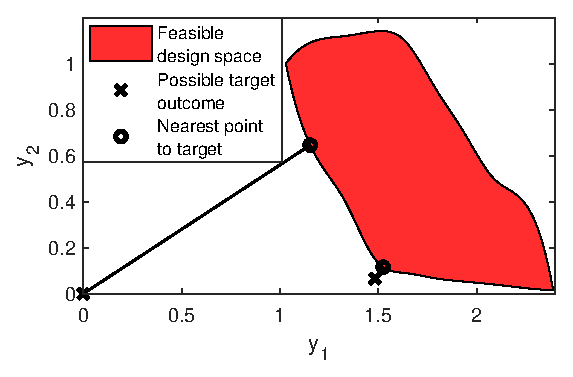
\includegraphics[scale=.85]{FIG_des_obs_selection_example2}
	%\captionsetup{width=.4\linewidth}
	\if1\diss\captionsetup{width=.85\linewidth}\fi
	\caption{Two choices of target outcomes for CTO, drawing the posterior predictive distribution to two different regions of the feasible design space.}
	\label{fig:do_selection_example}
\end{figure}
%
Suppose that, prior to undertaking CTO, we know only that the model outputs are positive and the goal is to simultaneously minimize the competing objectives.
%
Then $(0,0)$ is a natural choice as a target outcome, despite the fact that it is not feasible.
%
% However, the optimal region determined by the choice of $(0,0)$ in this case is somewhat arbitrary.
%
%Notice that in this example the entire ``left'' and ``bottom''  edges of the design space comprise the Pareto front.
%
The point closest to $(0,0)$ is unique in the Pareto front solely in being nearest to the origin, and that choice of target outcome was itself driven merely by our ignorance of the feasible design space.
%
%Thirdly, since we don't know the range of the feasible design space, we are not able to set an informative prior for $\lambda_\delta$.
%
By contrast, suppose now that preliminary CTO has supplied us a rough estimate of the Pareto front, empowering us to choose a different target outcome. For instance, $(1.32,0.065)$ targets a point of diminishing returns in allowing $y_1$ to increase further in exchange for a reduced $y_2$.
%
%Firstly, each point is much closer to the design space, leading to greater identifiability.
%
%Secondly, these choices of target outcome and resulting optima are not arbitrary, but rather are driven by articulable goals informed by an estimate of the Pareto front.
%
%Thirdly, with a rough estimate of the Pareto front we can supply a strong (or even degenerate) prior for $\lambda_\delta$.
%
Note also that when an emulator is used, preliminary CTO can use the same model observations as the subsequent CTO to train the emulator.
%
So preliminary CTO does not add to the budget of model runs, and is thus a computationally cheap supplement to CTO.
%

%
\section{Simulated Example}\label{example}
%

%
To illustrate our proposed procedure, we consider a version of the example problem ZDT1 described by \if0\diss Deb and Sundar\fi \cite{Deb2006a}.
%
For this illustration we have two objectives $y_1, y_2,$ and five design variables $\boldsymbol\theta=(\theta_1,\theta_2,\ldots,\theta_5)$ with $\theta_i\in[0,1]$ for all $i$.
% 
We seek optimal settings for $\boldsymbol\theta$.
%
Model outputs are $y_1 = \theta_1$ and $y_2 = g(1-\sqrt{\theta_1/g})$, where $g=1 + \frac{9}{4}\sum_{i=2}^5\theta_i$.
%
Though in reality each output is in the range $[0,1]$, we assume the vague prior knowledge only that the outputs are each in the range $[-6,\infty)$.
%
Figure \ref{fig:toy_sim_outputs} displays the (normalized) outputs as functions of $\theta_1$ and $\theta_2$ at $x = 2$, where $\theta_i=0$ for $i=3,4,5$.
%
\begin{figure}
	\centering
	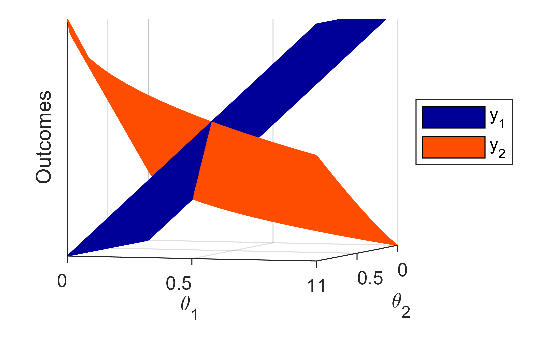
\includegraphics[scale=.85]{FIG_ZDT_model_outputs.eps}
	%\captionsetup{width=.4\linewidth}
	\if1\diss\captionsetup{width=.85\linewidth}\fi
	\caption{True two-dimensional profile outputs of the five-dimensional simulated example model.}
	\label{fig:toy_sim_outputs}
\end{figure}
%
Assuming an easily evaluated model (so that an emulator is not needed), we have
%
$
\mathbf z(x) = \eta(\boldsymbol \theta) + \boldsymbol\epsilon
$
%
for target outcome $\mathbf z$, so that  $\boldsymbol\eta = (y_1,y_2)^T$ is the output and $\epsilon_i\sim N(\mathbf 0,\sigma_i^2), ~i=1,2$.
%
For this example we set the prior $\sigma^2_i$ to be exponential distributions with mean 0.001 for $i=1,2$, corresponding to prior information that there is very little variation in the observed system outputs for a given design setting.
%

We initially set the target outcomes to $(0.25, -6)$, representing a target chosen with very little knowledge of the location of the system Pareto front. 
%
%This confidence is based on the observation that 
%since $F(\mathbf x-(0.71,0.71,17.92)^T)>0.95$, where $\mathbf x$ is the nearest point of the estimated Pareto front and $F$ is the cdf of the tolerance $\boldsymbol\epsilon\sim N(\mathbf 0, 0.05I)$.
%
For comparison, we also performed CTO with target $(0.3984, -2.1501)$, which lies much closer  to the feasible region (two standard deviations away, under a uniform prior on $\boldsymbol\theta$, compared to the original target's 5.2), on the line connecting the original target point to the nearest point in the feasible objective space.
%
%
Figure \ref{fig:toy_sim_results} shows the resulting posteriors of $\theta_1$ and $\theta_2$. % of the two design procedures, including the marginal distributions of the design variables. 
%
The marginal posteriors of the remaining inputs are practically  indistinguishable from those of $\theta_2$ and thus are not shown.
%
In the top plot, the original target is just over 5.2 units away from the objective space, where each objective is standardized to have variance 1.
%
In the bottom plot, the Euclidean distance of the target from the objective space is 2.
%
The posteriors are similar in the two cases, demonstrating that the method is not sensitive to differences in the distance of the chosen target from the feasible objective space.
%
The marginals in each case show substantial Bayesian learning compared to the prior (uniform) distribution of the design variables. 
%
CTO successfully maps the contours of the optimal region in each case, peaking near the true optimum. 
%
%Thus this bias with respect to the true optimum of the system is representative of the methodology's robustness with respect to remaining uncertainty in the values of $\theta_i$ for $i=2,\ldots,5$.
%
This example demonstrates the robustness of CTO to the distance between the target outcome and the feasible objective space.
%
Thus, a target outcome can be selected even when little is known about the location of the Pareto front.

%
\begin{figure}
	\centering
	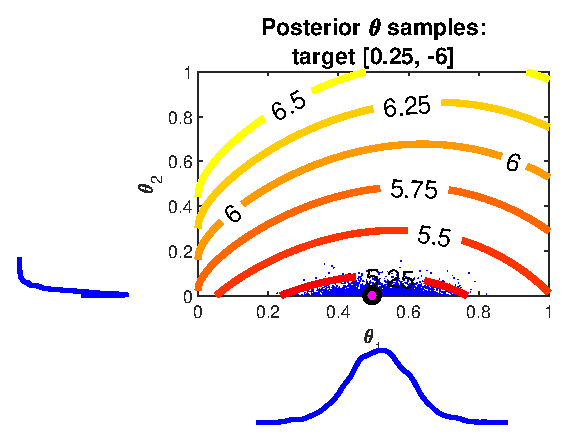
\includegraphics[scale=.85]{FIG_ZDT_results_5p222SD}\\
	\vspace{1em}
	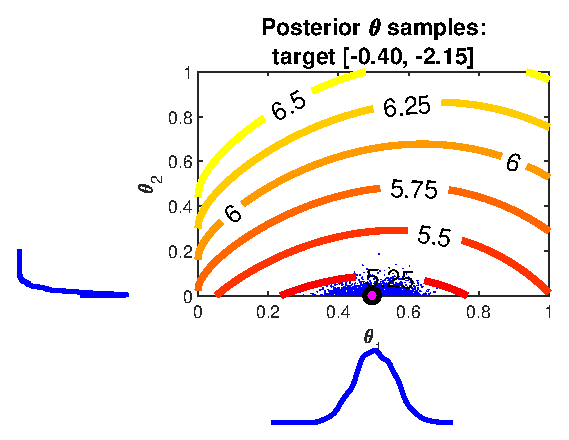
\includegraphics[scale=.85]{FIG_ZDT_results_2SD}
	%\captionsetup{width=.7\linewidth}
	\if1\diss\captionsetup{width=.85\linewidth}\fi
	\caption{Posterior draws from CTO in the simulated example using an arbitrary (non-feasible) point as a target (top) and using an updated target designed to lie two standard deviations from the Pareto front, in the direction of the original target (bottom). The contours show, for each point in the design space, the Euclidean distance of the model output at that point from the original target point $(0.25,-6)$, when $\theta_i=0$ for $i=3,4,5$ (which is the optimal setting for those inputs). The large dot shows the true optimum.}
	\label{fig:toy_sim_results}
\end{figure}



\section{Wind turbine material design application}\label{application}

In this section we use CTO to customize a material for use in a wind turbine blade. % of fixed geometry. 
%
The material is to be designed specifically for the end use of optimizing blade performance.
%
 
%HERE


\subsection{Wind turbine blade design}

The two blade performance measures of interest here are tip deflection and twist angle.
%
The engineering design goal is to keep these measures low while also minimizing material cost.
%
The blade is a composite of a given matrix and filler. 
%
%In a composite, the matrix holds the filler together; for example in concrete, a filler of loose stones combines with a cement matrix.
%
The material properties (and thus blade performance and cost) depend on the thickness of the shear web in the blade and on the volume fraction, or ratio of filler to matrix.
%
%The resulting material properties impact the performance and cost of the blade. 
%
Temperature also affects the composite's properties and hence its performance. It is a known operating condition of the blade but of course is not controllable. Hence, we treat temperature as an operational domain input but not a design parameter in the computer model. 
%
The model inputs are a triplet $(h,v,k)$, where $h$ is the temperature of the turbine (in kelvin), $v$ is the volume fraction, and $k$ is the thickness (in mm). 
%
The model output is a triplet $(d,r,c)$, where $d$ is tip deflection (in meters), $r$ is twist angle (in radians), and $c$ is cost per square meter (USD) of the material.
%
The turbine is deemed to operate over temperatures 230K-330K. 
%

%We used CTO to find a distribution on optimal settings for $v$ and $k$ given outputs from the finite element simulator and target outcomes.

\subsection{Emulation of finite element model}\label{emulator} %HERE 
The finite element model is one developed at Sandia National Laboratory for the CX-100 blade. We use \texttt{ANSYS} finite element analysis software \if1\diss\citep{ansys}\else\cite{ansys}\fi, interfaced with \texttt{MATLAB} \if1\diss\citep{MATLAB2017} \else\cite{MATLAB2017}\fi code and the \texttt{NuMAD} \if1\diss\citep{BergResor12} \else\cite{BergResor12}\fi manufacturing design tool.
The finite element model's estimations of material properties are based on the Mori-Tanaka model \if1\diss\citep{Mori1973}\else\cite{Mori1973}\fi.
Details of the blade and the finite element model may be found in the Appendix. We assume the finite element model accurately represents reality \if1\diss\citep{VanBuren2013,VanBuren2014}\else\cite{VanBuren2013,VanBuren2014}\fi. 

The finite element simulator is too computationally expensive to be suitable for direct use in an MCMC routine. 
%
To train the GP emulator, we drew 30 (trivariate) observations from the finite element simulator according to a Latin hypercube sampling design \if1\diss\citep{McKay1979} \else\cite{McKay1979}\fi based on plausible ranges for the three inputs as identified by subject matter experts: $[230\mathrm{K}, 330\mathrm{K}] \times [0.2, 0.6]\times[10\mathrm{mm},25\mathrm{mm}]$.
%
We used a GP with mean 0 and product power exponential covariance function as given in Equation \eqref{eq:Hig_cov}.
%
The GP emulator was validated using 10-fold cross-validation and determined to be an adequate surrogate for the FE model with 30 training points. In fact, there was little difference in predictive ability between 30 and up to 500 training points. Details of the validation of the emulator are in the Appendix.
%
% Though we employed the full 500 observations that were available to us, the emulator was found to be accurate when trained with far fewer samples, with only modest decrease in performance when using as few as 30 observations.
%

%
The hyperparameters $\lambda_\eta,\boldsymbol \beta^\eta$ are estimated %to plug in to the prior
% 
%To avoid our estimates being biased by the influence of the target outcomes, we estimated them prior to the design stage 
via maximum likelihood using only the finite element model output.
% 
%Initially, a grid optimization method was used: a grid of $\boldsymbol \beta^\eta$ values was used, finding at each point of the grid the likelihood of the simulation observations integrated over the support of $\lambda_\eta$. 
%
%However, $\boldsymbol \beta^\eta$ is a five-dimensional vector, and a grid fine enough to be useful was too computationally burdensome to be feasible. Instead, a 
We used \texttt{fmincon()} in \texttt{MATLAB} \if1\diss\citep{MATLAB2017} \else\cite{MATLAB2017}\fi %\cite{Cauchy1847} 
to maximize (with $D=\boldsymbol\eta$) over the joint (four-dimensional) support of $\boldsymbol \beta^\eta,\lambda_\eta$.  
%
The estimated values are shown in Table \ref{table:mles}.
%
\begin{table}[h]
	\renewcommand{\arraystretch}{1.2}
	\begin{center}
		\begin{tabular}{|c|c|c|c|}
			\hline 
			& $d$ & $r$ & $c$ \\ 
			\hline 
			$\hat\rho^\eta_h$	&0.7239 & 0.7104  & 1 \\ 
			\hline 
			$\hat\rho^\eta_v$	&0.9788&  0.9723  & 0.9988 \\ 
			\hline 
			$\hat\rho^\eta_k$	& 0.9906 &0.9882  & 0.9986 \\ 
			\hline 
			$\lambda_\eta$	& 0.0177  & 0.0261 & 0.0009 \\ 
			\hline 
		\end{tabular} 
	\end{center}
	\if1\diss\captionsetup{width=.85\linewidth}\fi
	\caption{Covariance hyperparameter maximum likelihood estimates for each objective function in the turbine blade example, obtained from 30 training computer runs. For each objective and each input $i$, $\rho_i^\eta = \exp(-\beta^\eta_i/4)$. The objectives are deflection $d$, rotation $r$ and cost $c$.}
	\label{table:mles}
\end{table}
%

\subsection{Design of the wind turbine blade system}\label{the_model}
%
All model inputs were rescaled to [0,1]. 
%
All model outputs were standardized so that each of the three responses had mean 0 and standard deviation 1.
%
% The full joint posterior density of the design variables and discrepancy function hyperparameters is given in Equation \eqref{eq:full_dist}, using the MLEs given above.
%
Initial target outcomes were set to the estimated utopia point $(0.6551\mathrm{m},\ 0.0768\mathrm{rad},\ \$96.8)$ found by taking the minimum observed value of each objective from the 30 simulator observations. 
%
The target was replicated to be constant as a function of temperature over an evenly-spaced grid of temperature values between 230K and 330K.
%

We carried out preliminary CTO with $\boldsymbol\sigma^2=5\times10^7\cdot(1,1,1)$ to estimate the Pareto front and locate a region of interest. % and thereby improve identifiability of the optimal region.
%
6,000 iterations were drawn via Metropolis-Hastings-within-Gibbs MCMC \if1\diss\citep{Metropolis1953, Hastings1970, Geman1984} \else\cite{Metropolis1953, Hastings1970, Geman1984}\fi in each of three chains (with random starts), of which the first 3,000 were discarded as burn-in. 
%
During the burn-in period, the covariances of the proposal distributions were periodically adjusted to be the sample covariance of the preceding draws scaled for an optimal acceptance rate of around $23\%$ for the multivariate input space \if1\diss\citep{Roberts1997,Gelman2013}\else\cite{Roberts1997,Gelman2013}\fi.
%
%The adjustment took place every 100 iterations of the MCMC, at which point the relevant covariance matrix was set to be equal to the sample covariance of the previous draws, times a scalar multiplier. 
%
%The level of the scalar multiplier was adaptively adjusted to promote optimal acceptance rates of $\approx 30\%$ for $\boldsymbol\theta$ and $\boldsymbol\rho$, and $\approx 44\%$ for $\lambda_\delta$.
%
Convergence of the three chains was verified visually and by the Gelman-Rubin statistic \if1\diss\cite[$\approx1.01$;][]{Gelman1992a}\else($\approx1.01$ \cite{Gelman1992a})\fi.
%

%
As expected for preliminary CTO, the posterior distribution of $\boldsymbol\theta = (v, k)$ was quite diffuse.
%
We used the GP emulator to predict the model output for each realization of $\boldsymbol \theta$.
%
Figure \ref{fig:elbow} displays the estimated Pareto front after filtering the posterior predictions to retain only non-dominated performance predictions.
%
Though the objective space is three-dimensional, the Pareto front appears to be a roughly coplanar curve describing a trade-off between cost and deflection/twist.
%
A distinct "knee point" of maximum curvature appears in the Pareto front. 
%
This seems to be a point of diminishing returns in the trade-off between performance and cost, and thus we selected this point as the target for design.
%
\begin{figure}
	\centering
	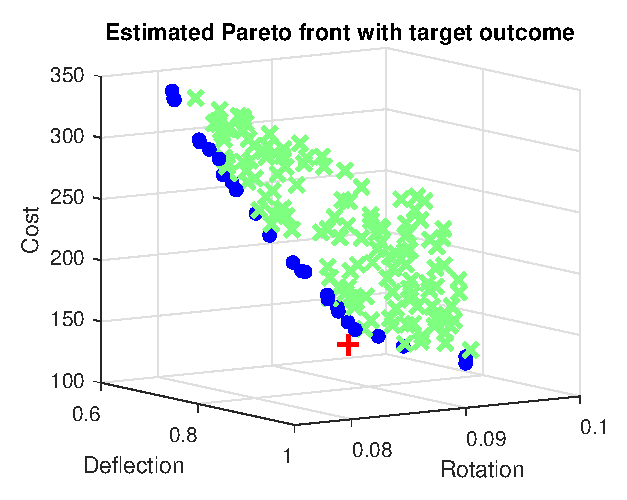
\includegraphics[scale=0.85]{FIG_est_PF_with_des_obs.eps}
	%\captionsetup{width=.7\linewidth}
	\if1\diss\captionsetup{width=.85\linewidth}\fi
	\caption{Each x is a dominated design drawn from the predictive distribution through preliminary CTO. The dots indicate the estimated Pareto front. The plus sign is the target selected as the performance objective in our proposed design approach.}
	\label{fig:elbow}
\end{figure}
%
To do so, we set the point $(\mathrm{deflection}=0.743\mathrm m,\ 
\mathrm{twist}=0.089\ \mathrm{rad},\ 
\mathrm{cost}=\$71.11)$
as the target outcome, replicated to be constant as a function of temperature as in the preliminary round.
%

%
In the subsequent CTO, we employed the same MCMC approach as in the preliminary round, except we now assign each element of $\boldsymbol\sigma^2$ an $\mathrm{Exp}(0.001)$ prior.
%
The covariances of the proposal distributions for each $\sigma^2_i$ were periodically adjusted to be the sample covariance of the preceding draws scaled for an optimal acceptance rate of around $44\%$ for the scalar $\sigma^2_i$ \if1\diss\citep{Roberts1997,Gelman2013}\else\cite{Roberts1997,Gelman2013}\fi.
%
The posterior distribution of $\boldsymbol\theta$ appears in Figure \ref{fig:wt_marg_post}, with a mode near $(0.6, 10\mathrm{mm})$.
%
Indeed, from the analysis discussed in Section \ref{removing_cal_pars}, we find that the ``knee point'' in the Pareto front is precisely the point at which volume fraction has reached its upper limit at $0.6$, with further gains possible only by raising thickness from its lower limit of $10$mm.
%
The contrast of the posterior distribution with the prior, which is uniform over $[0.2,0.6]\times[10,25]$, indicates that strong Bayesian learning has occurred.
%
%\begin{figure}
%\centering
%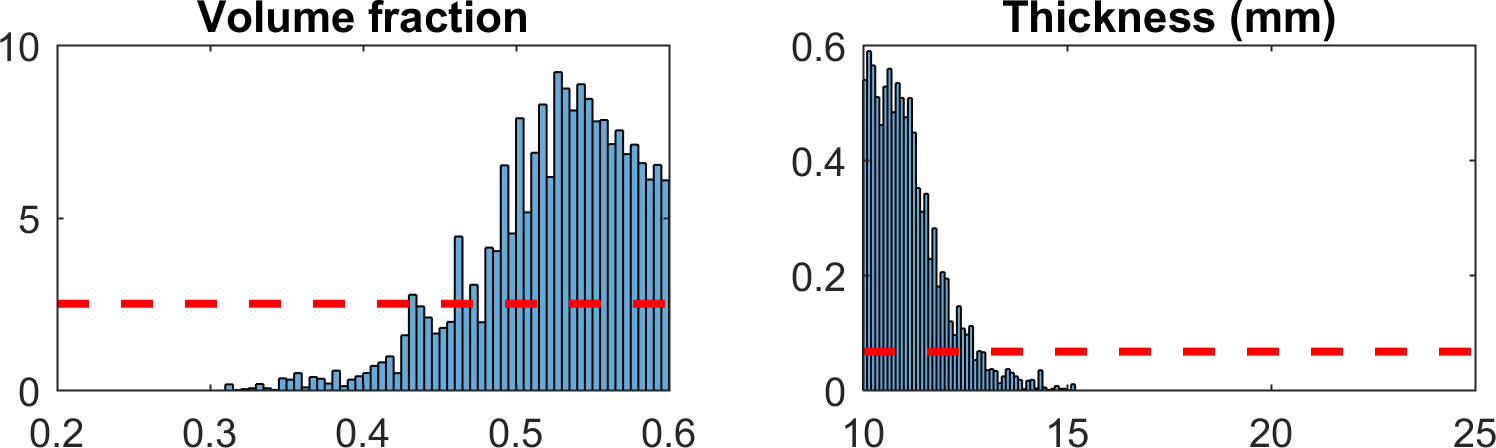
\includegraphics[width=.7\linewidth]{FIG_posterior_marginals_with_priors}
%\captionsetup{width=.7\linewidth}
%\caption{The histograms show the marginal posterior of each calibration parameter. The dotted lines show the priors.}
%\label{fig:wt_marg_post}
%\end{figure}
\begin{figure}
	\centering
	%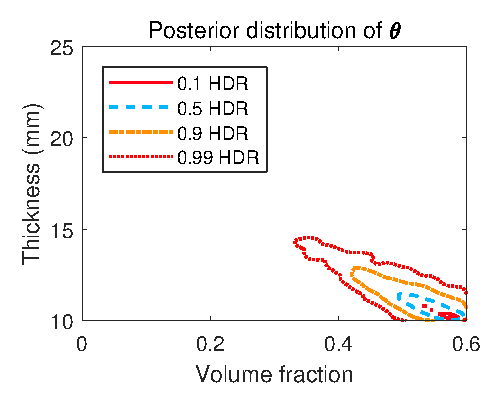
\includegraphics[width=.4\linewidth]{FIG_post_dist_contourplot}
	%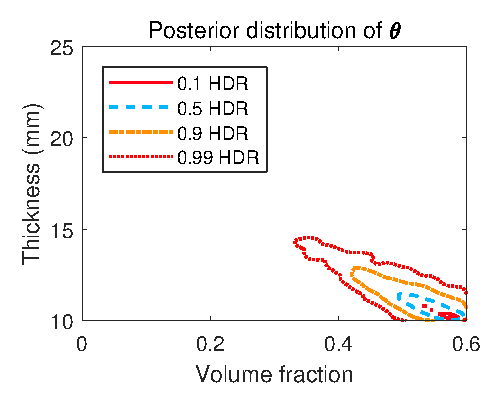
\includegraphics[scale=0.8]{FIG_post_dist_contourplot}
	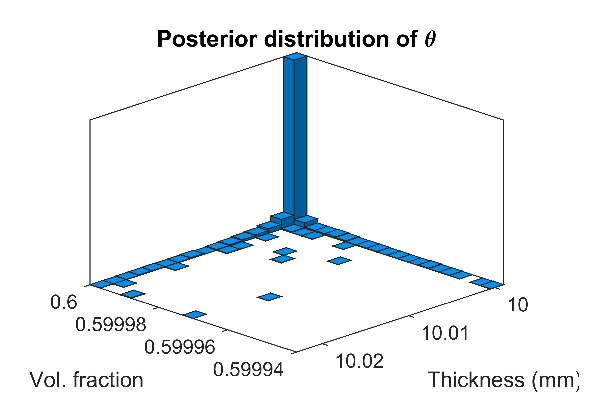
\includegraphics[scale=0.85]{FIG_post_dist_hist2}
	%\captionsetup{width=.7\linewidth}
	\if1\diss\captionsetup{width=.85\linewidth}\fi
	\caption{Histogram showing the posterior distribution from CTO in the wind turbine blade system. The prior is uniform over $[0.1,0.6]\times[10,25]$.}
	\label{fig:wt_marg_post}
\end{figure}
%
The prior and posterior predictive distributions of the model outputs appear in Figure \ref{fig:prior_post_pred_comp}, where the prior predictive distributions are based on a uniform sampling of the model inputs.
%
\begin{figure}[h]
	\centering
	%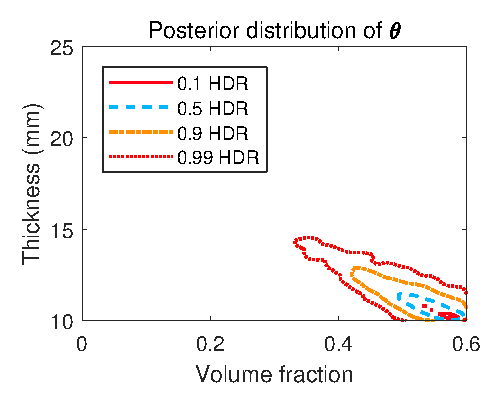
\includegraphics[width=.4\linewidth]{FIG_post_dist_contourplot}
	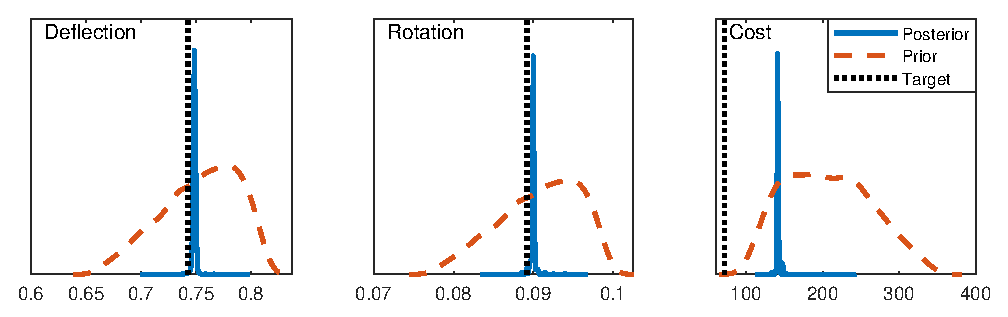
\includegraphics[scale=0.85]{FIG_prior_vs_posterior_dist}
	%\captionsetup{width=.7\linewidth}
	\if1\diss\captionsetup{width=.85\linewidth}\fi
	\caption{Approximate prior and posterior marginal predictive densities for each of the three outputs in the turbine blade design problem.}
	\label{fig:prior_post_pred_comp}
\end{figure}
% HERE
The mean output under the prior is $(0.753\mathrm m,0.091\text{ rads},\$206.58/\mathrm m^2)$, and under the posterior it is $(0.751\mathrm m,0.090\ \mathrm{rad},\$139.80/\mathrm m^2)$.
%
Though the mean performance outcomes are approximately the same under the posterior and the prior, mean cost per square meter and the uncertainty of the outcomes are dramatically lower.
%
If one prefers to prioritize gains in performance over cost, this can be accomplished by selecting target outcomes that reflect those priorities.
%

%
\subsection{Pareto front estimation with quantified uncertainties}\label{removing_cal_pars}

%\subsubsection{Motivation}

%Often in the case of a system with multivariate output, one might not antecedently have a clear goal for design.
%
%All else being equal, w
When multiple design outputs are to be minimized, any point in the Pareto front is optimal relative to some set of priorities.
%
If those priorities have not been explicitly determined prior to the design process, then no particular outcome can be targeted.
%
%In determining one's priorities, it is helpful to know the Pareto front of the relevant system.
%
For example, in a system where performance is monotonically increasing in cost, depending on one's tolerance for high cost, any point in the design space might be optimal.
%
%In determining one's priorities and selecting a target outcome, it is valuable to have a clear and accurate understanding of the Pareto front of the system.
%
In low-dimensional cases, CTO may be used to achieve a holistic picture of the Pareto front by optimizing to each target outcome on a grid.
%
To do this, where the model output is $b-$dimensional, one may draw a grid over the range of $b-1$ of the model outputs and perform CTO to minimize the remaining output at each point of the grid.
%
The $b-1$ outputs, at each grid point, are treated as known up to small error (e.g., one tenth of one standard deviation from the mean).
%
Allowing some small observation error is necessary because any set of solutions having Lebesgue measure zero has probability zero of occurring.
%
The resulting estimate of the Pareto front differs from the filtering method employed in preliminary CTO in that it allows for quantifying the uncertainty associated with the Pareto front.
%

%
Our proposed procedure is illustrated here using the wind turbine blade application.
%
For ease of exposition, twist has been removed as a model output, leaving a system with two-dimensional output of deflection and cost. 
%
The range of observed costs is $[\$96,\$286]$.
%
A 20-point grid was drawn over this range of costs. 
%
%Using the rough estimate of the Pareto front from preliminary CDO, we found that to cover the Pareto front, the cost grid should cover the range $[\$96,\$352]$.
%
For each point $c$ in the cost grid, we used the point $(0\mathrm m,\$c)$ as the target outcome for calibration (again replicated as constant with respect to temperature). The result is an estimate of the response surface with quantified uncertainty describing, for each point in the grid, the minimal achievable outcome for the output not included in the grid.
%

%

%
%This enables a decision-maker to visualize the space of desirable possibilities with associated uncertainties. 
%
%They can do so without the need for rigorously predetermining their exact priorities for weighing gains in each of the outputs against one another.
%
The result of applying this strategy to the wind turbine blade application is shown in Figure \ref{fig:known_cost}. 
%
\begin{figure}[h]
	\centering
	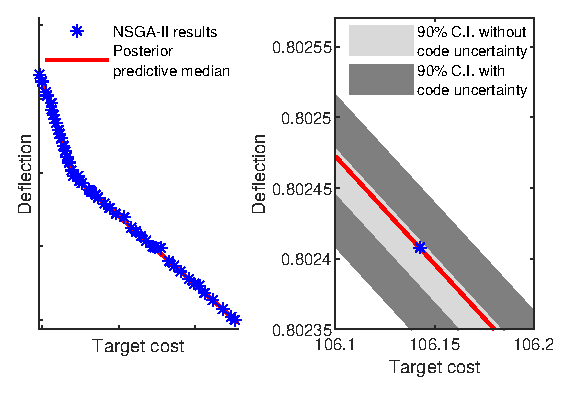
\includegraphics[scale=.85]{FIG_cost_grid_pareto_bands}
	%\captionsetup{width=.7\linewidth}
	\if1\diss\captionsetup{width=.85\linewidth}\fi
	\caption{The estimated Pareto front of the wind turbine blade system with quantified uncertainties, along with NSGA-II estimation of the front. The light gray shows the 90\% credible interval for the front without code uncertainty (i.e., treating the emulator as perfect); the dark gray extends the credible interval to include code uncertainty.}
	\label{fig:known_cost}
\end{figure}
%
% The lefthand plot shows the estimated Pareto front for the system.
%
For comparison, we also plot the results from applying the NSGA-II algorithm \if1\diss\citep{Deb2002}\else\cite{Deb2002}\fi, a popular gradient-free genetic algorithm for MOO. It uses the trained GP emulator as the objective function, with 500 generations and population size 50.
%
NSGA-II and our approach give very similar estimates of the Pareto front's location.
%
On a machine with an Intel Core i7-9750H CPU and 16GB of RAM, NSGA-II required 132 seconds.
%
While our method required more computation time (461 seconds), it generated far more informative results.
%
In contrast with that of NSGA-II, our approach can quantify all the sources of uncertainty. Such uncertainty is important to account for since no emulator is \textit{identical} to the computer model output, and because uncontrollable factors can affect performance (e.g., uncontrollable operating temperature that changes day to day).
%
%This plot visualizes a distribution on the optimal performance outcome for any cost that a decision-maker might select as a budget for production, which would be helpful when selecting a budget.
%
%For example, the point of maximum curvature around \$140 manifests itself as a potentially attractive choice, since it can be seen in the plot that prior to that point each dollar spent brings significant gains in reducing deflection.
%
%Spending above that level continues to reduce deflection, but less sharply.

%
Figure \ref{fig:more_pfs} shows the application of CTO to three different problems with a training set of 100 FE model runs each. 
%
\begin{figure}[h]
	% \centering
	\if1\diss
		\begin{tabular}{m{2.4cm}m{.3cm}m{2cm}}
			&(a)&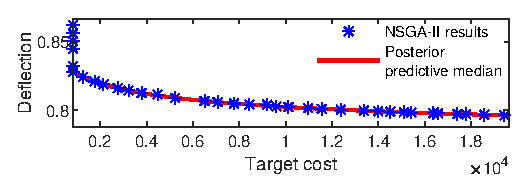
\includegraphics[scale=.85]{FIG_cost_grid_pareto_bands1}  \\
			&(b)&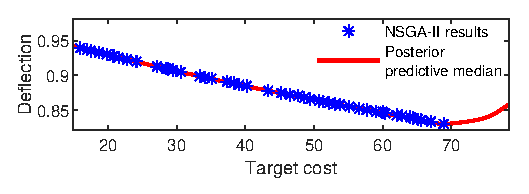
\includegraphics[scale=.85]{FIG_cost_grid_pareto_bands2}\\
			&(c)&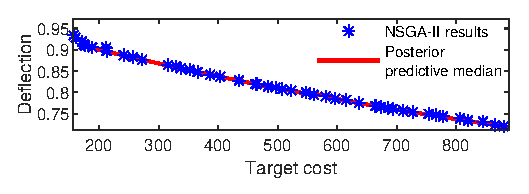
\includegraphics[scale=.85]{FIG_cost_grid_pareto_bands3}
		\end{tabular}
	\else
		\begin{tabular}{m{.3cm}m{2cm}}
		     (a)&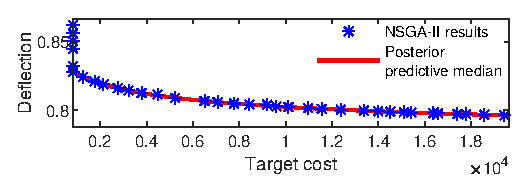
\includegraphics[scale=.85]{FIG_cost_grid_pareto_bands1}  \\
		     (b)&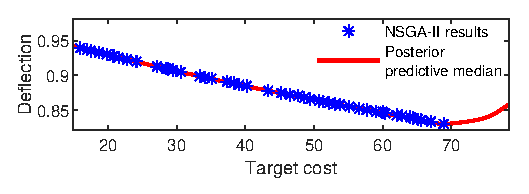
\includegraphics[scale=.85]{FIG_cost_grid_pareto_bands2}\\
		     (c)&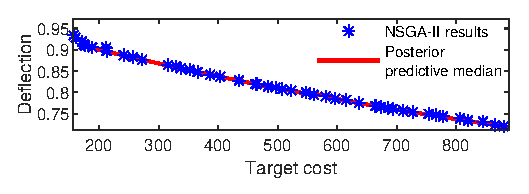
\includegraphics[scale=.85]{FIG_cost_grid_pareto_bands3}
		\end{tabular}
	\fi
	%\captionsetup{width=.7\linewidth}
	\if1\diss\captionsetup{width=.85\linewidth}\fi
	\caption{Estimated Pareto front for multiple wind turbine blade systems with respect to a variety of design spaces, along with NSGA-II estimation of the fronts. 95\% credible intervals are too small to be visible.}
	\label{fig:more_pfs}
\end{figure}
%
All three cases attempt bivariate minimization of both blade deflection and cost.
%
Subplot (a) searches for optimal design settings for the composite material's filler modulus and matrix modulus.
%
Subplot (b) searches for optimal aspect ratio and shear web thickness.
%
Subplot (c) shows the results for a search over three design variables: aspect ratio, volume fraction and shear web thickness.
%
In each case, CTO is consistent with the results from NSGA-II.
%
% Case (a) illustrates the danger that sharp changes in the front that take place in an interval much smaller than the CTO grid mesh size chosen can be missed by the procedure.
% %
% This can be avoided either by reducing the mesh size, or, alternatively, by using multiple CTO grids over different objectives -- e.g., in this case, minimizing cost over a grid of deflection amounts in addition to minimizing deflection over a grid of costs.
%
Notice also in Subplot (b) that CTO, in contrast with NSGA-II, is informative about the behavior of the system at costs beyond those in the Pareto front.
%

%
% The use of CTO in the wind turbine design problem illustrates how preliminary CTO may be used, not merely to improve the identifiability of a pre-determined optimal region as in Section \ref{example}, but rather to identify a desirable region of the design space and select target outcomes that design to that region.
% %
% In the wind turbine case, selecting the utopia point as one's target determines the optimal region to be the high-cost region toward the upper-left of Figure \ref{fig:elbow}, since (on the standardized scale of model outputs) that region happens to be closest to the target.
% %
% If one has substantive goals that drive one to select that target, then one is well-served by optimizing to that high-cost region.
% %
% But if the utopia point is chosen arbitrarily, then the resulting optimal region is itself determined arbitrarily.
% %
% The estimate of the Pareto front provided by preliminary CTO allows us to identify regions of special interest, and to select target outcomes that that lead to clearly defined designs, as illustrated in Figure \ref{fig:elbow}.
%

%
The use of CTO in this case demonstrates the value of obtaining a posterior distribution on the design variables, rather than just a point estimate.
%
For example, Figure \ref{fig:wt_marg_post} shows not just that a reasonable point estimate of the optimal $\boldsymbol\theta$ is at (0.6, 10mm)---respectively the upper and lower extrema of the supports for volume fraction and thickness. We also have information about the variation in the design space corresponding to variation in the observed performance from one experiment to the next.
%
This is potentially useful for studying system tolerances.
%

The wind turbine case illustrates how our proposed method can deliver ``Pareto bands," providing not merely an estimate of the Pareto front (as in preliminary CTO) but also uncertainty associated with that estimate.
%
Such an estimate can be of use to decision-makers when deciding on performance goals subject to budgetary constraints while also accounting for uncontrollable factors in the manufacturing process or operating environment.



\section{Discussion} \label{conclusion}
% Discussion of the role of computer model validation as a potential methodology for design

We have described how the 
%theoretical background for the use of Gaussian processes to emulate computationally expensive computer model code, and the 
computer model calibration framework of \cite{Kennedy2001} can be adapted for engineering design. 
%
Calibration to target outcomes undertakes design by ``calibrating'' a model not to field observations, but rather to performance and cost targets. 
%
The procedure optionally includes a computationally cheap preliminary step that provides a rough estimate of the Pareto front, which may be used to select target outcomes that promote strong Bayesian learning.
%
The resulting posterior predictive distribution approximates the target outcomes, so that the posterior distribution of $\boldsymbol\theta$ constitutes a distribution on optimal design settings.
%
Repeated applications of this methodology allows one to construct a thorough estimate of the Pareto front of the system with quantified uncertainties by selecting target outcomes that explore different portions of the Pareto front.

Unlike other methods of Bayesian optimization \if1\diss\cite[a review of which is provided by][]{Shahriari2016}\else(a review of which is provided by \cite{Shahriari2016})\fi, CTO does not require the ability to evaluate model output adaptively.
%
Instead, it can rely on a batch of observations gathered prior to (and independently of) the design process.
%
We described the implementation of this approach in an MCMC routine along with considerations to accommodate computational instability.
%
The use of this methodology is illustrated in the case of material design for a wind turbine blade. 
%
%We have shown thereby a variety of ways in which CTO can be used to guide decision-makers in the design process. 
%
By expropriating established tools of model calibration, CTO offers a method of optimization which is sensitive to, and quantifies, all sources of uncertainty.
%

%
The example of Section \ref{example} has five design inputs and bivariate objectives, and the applications in Section \ref{application} each had either two or three design inputs and two or three objectives.
The number of objectives is mostly for ease of illustration and visualization, as well as practical interest in the turbine blade design problem. There exist many design problems with many more objectives and/or design dimensions than those considered here. 
In considering the computational burden associated with a larger number of objectives, we follow standard practice by assuming independent Gaussian processes for each output \if1\diss\citep{Picheny2015}\else\cite{Picheny2015}\fi, meaning that the computation essentially scales linearly with the number of outputs. For cases in which independent GPs are not appropriate, it is certainly possible to account for the dependence of the outputs in the surrogate model \if1\diss\citep{ContiOHagan10}\else\cite{ContiOHagan10}\fi. 
The computational burden of such an approach would be more severe in such a case. While CTO with a {\em single} target can be applied with larger numbers of objectives, the grid-based Pareto front estimation can become prohibitive since the required grid grows exponentially with the dimension of the objective space. With respect to the dimension of the design space, the limitations of CTO here are those that arise from the underlying MCMC algorithm. High-dimensional MCMC is the subject of ongoing research, some of which is reviewed \if1\diss by \cite{SaibabaEtAl19}\else in \cite{SaibabaEtAl19}\fi. 
While an exploration of this issue is beyond the scope of the current work, we remark that marginalization and Hamiltonian Monte Carlo have been shown to be effective. Another partial remedy for these difficulties would be to perform an \textit{a priori} sensitivity analysis in order to reduce the inputs only to those that substantially affect the output. Similarly, one could use active subspaces \if1\diss\citep{Constantine2015} \else\cite{Constantine2015}\fi to reduce the dimensionality of the design space.

It is possible for there to be proper subsets of the design space that are not feasible (e.g., design values that cannot be meshed for shape optimization), or that are poorly identified by the performance criteria (i.e., an ill-posed inverse problem). The Bayesian approach that we use here is naturally suited for such situations. For example, the prior on the design space can place zero probability on infeasible subsets or otherwise impose regularization to constrain the space of possible solutions. This latter feature is one of the reasons the Bayesian approach to inverse problems has been gaining popularity over the last few years \if1\diss\citep{Calvetti2014}\else\cite{Calvetti2014}\fi.

%

The example and applications we describe here correspond to unconstrained problems. However, methods are available for constructing GPs that incorporate known constraints. For example, \if0\diss Golchi et al. \fi\cite{Golchi2015} use sequential Monte Carlo to simulate GPs that are monotone with respect to some or all inputs. 
\if0\diss Wang and Berger \fi\cite{Wang2016} similarly discuss methods for incorporating shape constraints (including monotonicity) into a GP. 
\if0\diss Maatouk and Bay \fi\cite{Maatouk2017} use a functional decomposition to create a finite-dimensional approximation of a GP that allows one to incorporate inequality constraints.  
\if0\diss Ding et al. \fi\cite{DingEtAl19} allow for boundary constraints in GP emulation with a mean function that honors the information along with covariance functions that go to zero at the known boundaries. We suspect that it would be straightforward to incorporate such procedures into our proposed design approach.

%
The methodology as described here treats the computer model as universally valid over the domain of the design variables. 
%
Future work in this area will include the use of a discrepancy term capturing model bias.
%
%That is, while CTO as presented above includes $\delta(\cdot)$ to capture systematic discrepancy between the target outcomes and the true system, it assumes that the computer model is an unbiased estimate of the true system.
%%
%The inclusion of a second discrepancy term to capture systematic differences between the model and the observed reality would avoid this idealizing assumption.
%
Other possible extensions of our proposed methodology include its application to so-called ``state-aware calibration'' \if1\diss\citep{Atamturktur2015,Stevens2018,Brown2016}\else\cite{Atamturktur2015,Stevens2018,Brown2016}\fi, which would allow the optimal region of the design variables to vary as a function of the operational domain inputs.

%%%%%%%%%%%%%%%%%%%%%%%%%%%%%%%%%%%%%%%%%%%%%%%%%%%%%%%%%%%%%%%%%%%%%%
% \begin{acknowledgment}
% 	\thanks{
% 		The authors gratefully acknowledge grant CMMI-1934438 from the National Science Foundation (NSF). CE was supported by fellowships through Department of Education GAANN grant P200A150310 and NSF NRT grant 1633608. DAB is also supported by NSF grants EEC-1744497 and OIA-1826715.}
% \end{acknowledgment}

%%%%%%%%%%%%%%%%%%%%%%%%%%%%%%%%%%%%%%%%%%%%%%%%%%%%%%%%%%%%%%%%%%%%%%
% The bibliography is stored in an external database file
% in the BibTeX format (file_name.bib).  The bibliography is
% created by the following command and it will appear in this
% position in the document. You may, of course, create your
% own bibliography by using thebibliography environment as in
%
% \begin{thebibliography}{12}
% ...
% \bibitem{itemreference} D. E. Knudsen.
% {\em 1966 World Bnus Almanac.}
% {Permafrost Press, Novosibirsk.}
% ...
% \end{thebibliography}

% Here's where you specify the bibliography style file.
% The full file name for the bibliography style file 
% used for an ASME paper is asmems4.bst.
\if1\diss
\bibliographystyle{Chicago}
\bibliography{lit_review}
\else
\bibliographystyle{asmems4}
\bibliography{lit_review}
\fi


\pagebreak \pagebreak
\section*{Appendix}
\subsection*{Turbine blade finite element model}
The wind turbine blade model used in this paper is based on a nine-meter research and development blade developed by Sandia National Laboratory known as the CX-100 \if1\diss\citep{Berry08, BerryAshwill07}\else\cite{Berry08, BerryAshwill07}\fi. 
The purpose of the CX-100 blade is to provide an inexpensive test platform for structural modeling and strength testing and is comprised of a unidirectional carbon-fiber laminate with a fiberglass skin. 
Using the airfoil geometry and composite layer specifications described in the CX-100 development reports, the geometry of the blade is created using the NuMAD (``Numerical Manufacturing and Design") tool created by Sandia National Laboratories \if1\diss\citep{BergResor12, ResorPaquette12}\else\cite{BergResor12, ResorPaquette12}\fi. 
The NuMAD software serves to create the blade geometry based on input airfoil geometry data. Components of the blade (edges, root, spar caps, and shear web) are assigned composite material properties and geometry (layer orientation, quantity, and thickness). See Figure \ref{fig:bladeFig}.

\begin{figure}[h]
	\centering
	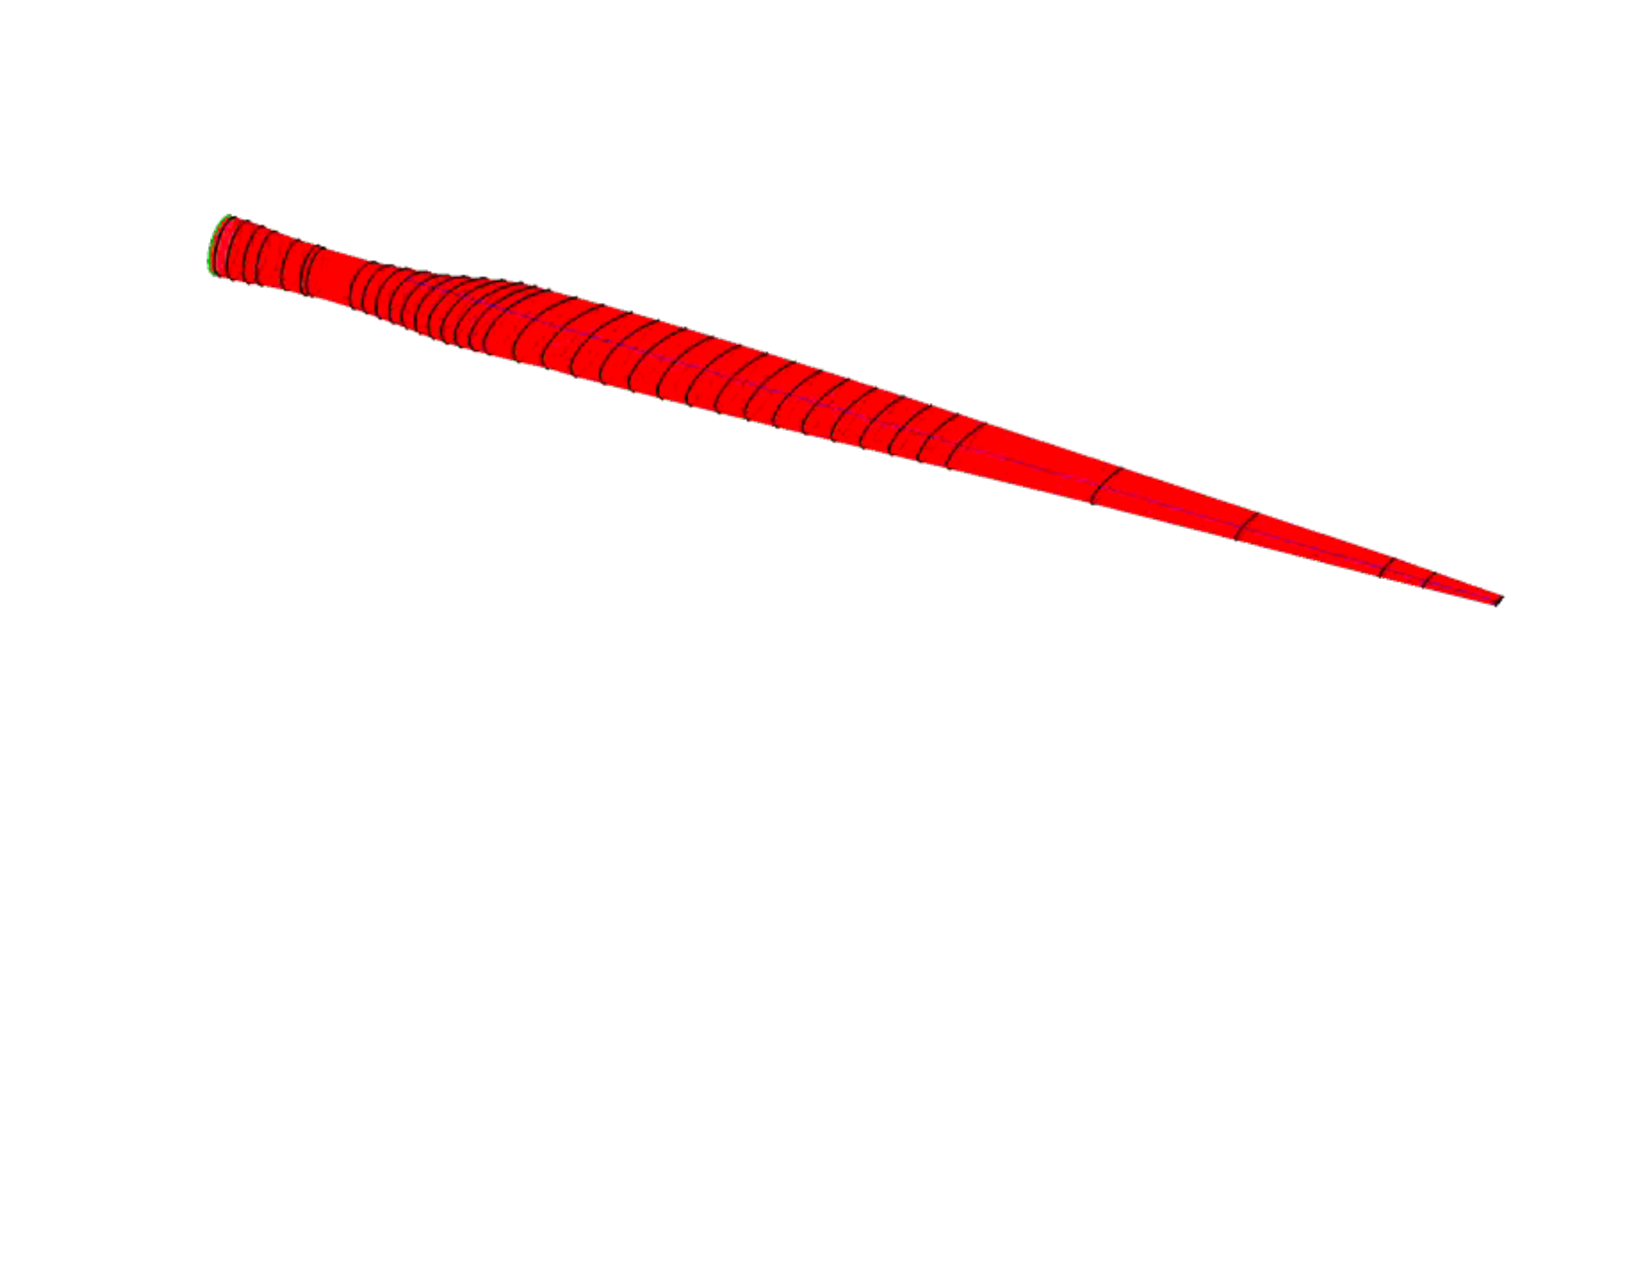
\includegraphics[scale=.25, trim= 0 3in 0 0]{BladeFig.pdf}
	%\captionsetup{width=.7\linewidth}
	\if1\diss\captionsetup{width=.85\linewidth}\fi
	\caption{CX-100 blade model created in NuMAD for ANSYS input file generation and finite-element analysis.}
	\label{fig:bladeFig}
\end{figure}

The NuMAD software is then used to export the created blade model as an ANSYS input file to create the geometry, mesh the body with the appropriate material properties and geometries, and apply the boundary conditions. The model is composed of 8-node structural SHELL281 elements in layers to represent the composite material layers and that support the application anisotropic material properties. The study uses fixed-free boundary conditions where the root is simulated to be fixed to the turbine hub and the tip is free to measure deflection due to loading. Loading is applied to the blade tip as a 6,000N load in the flapwise direction based on measured turbine hub moments of the same blade design under high wind loads of approximately 54,000 N-m. The ANSYS input is modified accordingly to apply the loading, solve the model, and export the nodal displacements and rotations.

\subsection*{Surrogate model validation}
The validation of the GP emulator was performed using 10-fold cross validation.
Figure \ref{fig:gp_validation} shows the results. 
Though we had access to a large set of 500 finite element model observations, we find that our GP emulator worked well for much smaller training sizes, as shown here. 
In each case, the RMSE for each of the three outputs is included.
Error bars for each observations are also included, but are generally too small to be visible. In each case, we see excellent agreement between the predicted and observed outputs.
This validation demonstrates the diminishing returns of using more than 30 finite element model observations to train the emulator.
\begin{figure}
	\centering
	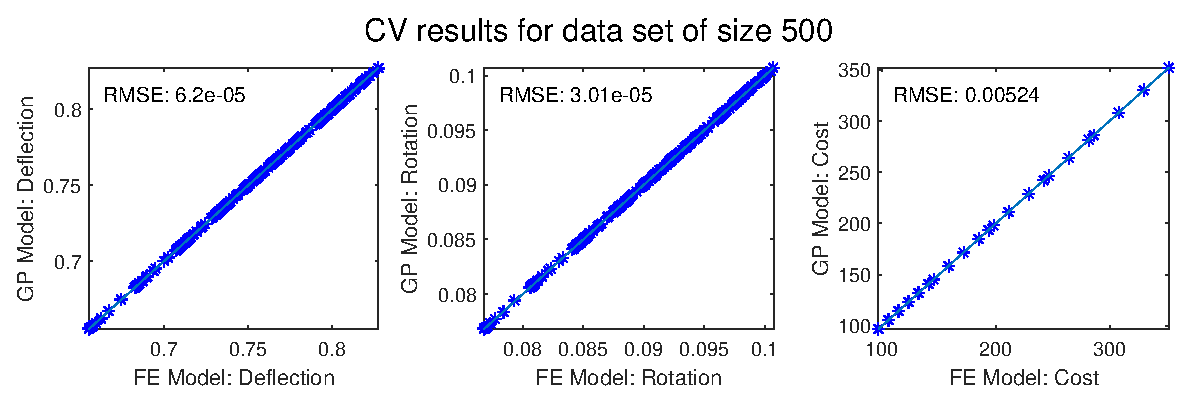
\includegraphics[scale=.45]{FIG_GP_CV_size500.eps}\vspace{1em}
	
	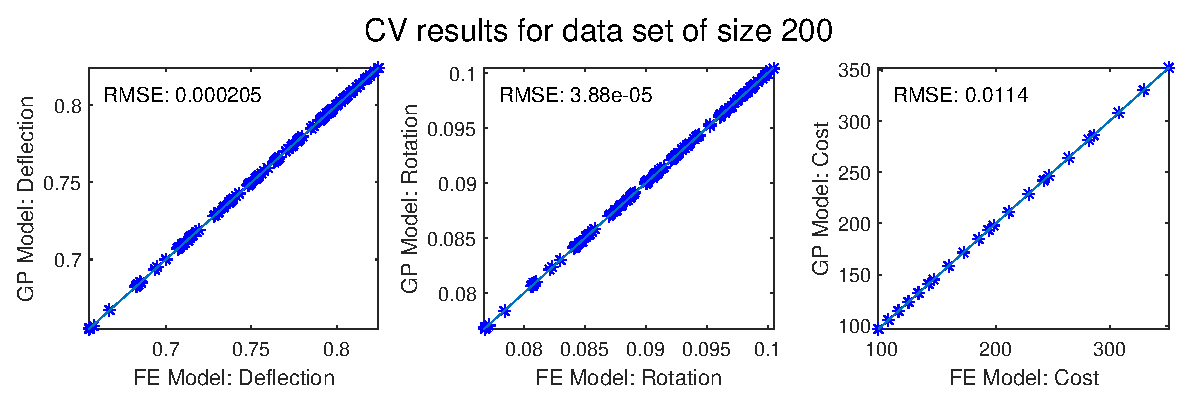
\includegraphics[scale=.45]{FIG_GP_CV_size200.eps}\vspace{1em}
	
	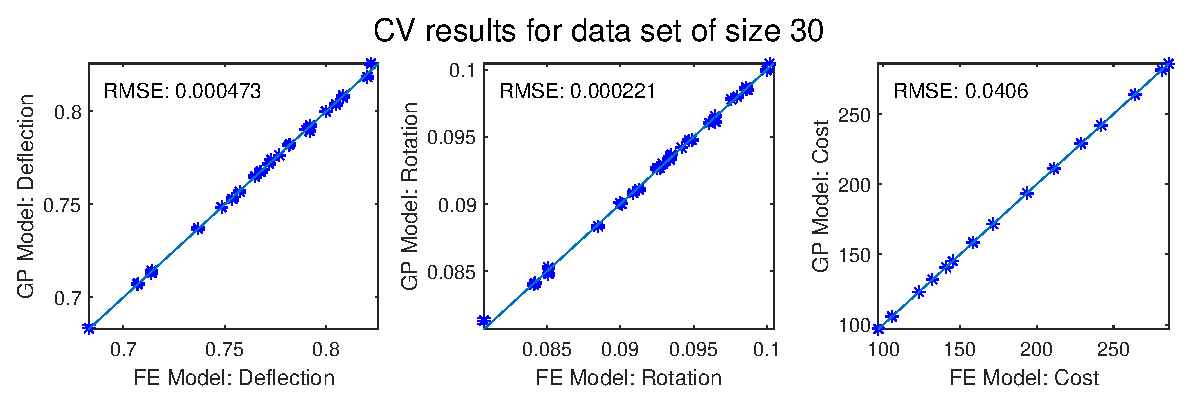
\includegraphics[scale=.45]{FIG_GP_CV_size30.eps}
	%\captionsetup{width=.7\linewidth}
	\if1\diss\captionsetup{width=.85\linewidth}\fi
	\caption{Results of 10-fold cross validation of the GP emulator used for the wind turbine application.}
	\label{fig:gp_validation}
\end{figure}

\end{document}
